\documentclass[
  a4paper,
  abstract=on,
  captions=tableabove
  ]{scrartcl}

%section{Ignore warnings}

  \usepackage{silence}
  \WarningFilter{latex}{Marginpar on page}

%section{Packages}

  \usepackage{packages}
  \addbibresource{~/promo/bib/references.bib}
  \usepackage{url}

  %subsection{extensions for the paper}

    \usepackage{siunitx}
    \sisetup{group-minimum-digits=4}

%section{New commands}

  \renewcommand{\hw}[1]{\textbf{#1}}

  \newcommand{\lsil}[1]{\lstinline[language=Python]{#1}}
  \newcommand{\mtrc}[1]{\textcolor{blue}{#1}}

  \newcommand{\sw}[1]{\texttt{#1}}

\begin{document}

% \begin{comment}

%section{Title}

  \title{Social networks of lexical innovation}
  \subtitle{Investigating the diffusion of neologisms on Twitter}
  \author{Quirin Würschinger\\ LMU Munich}
  \maketitle

%section{Todos}

  % \listoftodos

%section{Abstract}
  \cleardoublepage

  \begin{abstract}

    Societies continually evolve and speakers coin and use new words to talk about innovative products and practices. While most lexical innovations fail to catch on, others spread successfully and become part of the lexicon. This paper investigates the diffusion of English neologisms on Twitter. Previous work on lexical innovation has almost exclusively relied on usage frequency counts for measuring diffusion. Taking frequency as a baseline, I use social network analysis to zoom in on the sociolinguistic dynamics of diffusion.

    My results show that frequency counts lend themselves to approximate overall degrees of diffusion with varying success. While absolute counts can be misleading, incorporating temporal dynamics of use provides a better picture of diffusion. However, frequency-based information alone fail to capture important sociolinguistic characteristics. Social network information are shown to add valuable information about whether new words are known and used by an increasing number of individuals and communities of speakers. Firstly, I distinguish different pathways of diffusion depending on whether and to which degree new words show increasing vs. decreasing centralized use over time. Secondly, I show that social network information allow for a more fine-grained assessment of degrees of diffusion, for example when new words are used with increasing frequency when use their remains limited to certain parts of the speech community. Lastly, I compare the results based on usage frequency and on social network analysis. Besides notable discrepancies, we find a significant correlation between both types of information, which serves to cross-validate both approaches.

    My results suggest that social network information can complement frequency counts and that using information from both sources provides a more reliable and differentiated view of the sociolinguistic dynamics of diffusion. I argue that this is particularly important for investigating the diffusion of lexical innovations, as new words are often marked by high social indexicality and show substantial differences in use between communities of speakers. More generally, however, social network analysis shows great potential to study sociolinguistic dynamics of language variation and change beyong the domain of lexical innovation.

    \vspace{2\baselineskip}

    \textbf{Keywords}: lexicology, lexical innovation, sociolinguistics, diffusion, social media, Twitter, big data, social network analysis

  \end{abstract}

% text body

\section{Introduction}
  \label{sec:intro}

Societies continually evolve, new products and practices emerge, and speakers coin and adopt new words when they interact and share information. How do these new words spread in social networks of communicative interaction?

Covid-19 has recently spread through social contagion with shocking speed and has tragically affected the lives of people around the world. Its fatal consequences have demonstrated the devastating power of exponential diffusion in social networks. In a recent paper analysing contagion patterns of diseases in \emph{Nature Physics}, \textcite{Hebert-Dufresne2020MacroscopicPatterns} suggested that the spread of viruses follows principles of complex contagion through social reinforcement, and that it matches the dynamics of diffusion of cultural and linguistic innovations such as new words and internet memes. Does this confirm the widespread perception that new words \enquote{go viral}?

Influential sociolinguistic models of the spread of linguistic innovations like the S-curve model~\parencite{Milroy1992LinguisticVariation} share fundamental features with earlier economic models of diffusion~\parencite{Rogers1962DiffusionInnovations}, and such models show commonalities between the spread of cultural and linguistic innovations. It is often assumed that diffusion in social networks follows universal trajectories and that rates of spread depend on social dynamics such as network density and the presence or absence of weak ties~\parencite{Granovetter1977StrengthWeak}. Unlike research on biological and cultural diffusion processes, however, sociolinguistic research has only recently been provided with data sources that are equally suitable for large-scale, data-based approaches using social network analysis to study these phenomena empirically.

Social media platforms like Twitter have changed the way we communicate and how information spreads, and they offer large amounts of data for empirical research. Sociological research has been concerned with pressing issues regarding the impact of online social networks for the spread of hate speech, fake news and the power of \enquote{influencers}, bots and institutions on public opinions and elections, which increasingly strain the social fabric. For (socio-)linguists, social media provide large amounts of data of authentic language use which opens up new possibilities for the empirical study of language variation and change. The size of these datasets as well as their informal nature allow for large-scale studies on the use and spread of new words, for example, to gain insights about general trajectories~\parencite{Nini2017ApplicationGrowth} or about factors that influence whether new words spread successfully~\parencite{Grieve2018NaturalSelection}. Moreover, metadata about speakers allows studying aspects of diffusion that go beyond what can be captured by usage frequency alone. Recent work, for example, has used Twitter data to investigate the geographical spread of lexical innovations.~\parencite{Eisenstein2014DiffusionLexical,Grieve2017GeographicalPatterns,Grieve2018MappingLexical}

Data about the communicative interaction of speakers additionally allows performing network analyses of the social dynamics of diffusion processes. Network science approaches to social media data have been successfully employed in diverse fields, for example, to study the spread of diseases~\parencite{Lu2018AccurateInfluenza}, opinions~\parencite{West2014ExploitingSocial} and political attitudes~\parencite{PewResearchCenter2019NationalPolitics}. While the study of social networks has a long research tradition in sociolinguistics and has shaped influential models of diffusion~\parencite[e.g.][]{Milroy1985LinguisticChange}), large-scale network analyses of sociolinguistic phenomena have only recently become more widespread. These new data sources and methodological advances put computational sociolinguistics in an excellent position to gain new insights and to test long-standing theoretical models empirically.

In the area of lexical innovation, this can serve to evaluate important theoretical concepts like the role of early adopters, network density and weak ties \todo{references} in the diffusion of new words. For example, earlier approaches have used computational modelling to test the validity of the S-curve model~\parencite{Blythe2012ScurvesMechanisms}, and to model processes of simple and complex contagion of linguistic innovations in social networks~\parencite{Goel2016SocialDynamics}. Applying social network analysis to bigger samples of neologisms and tracking their diffusion on social media datasets promises to shed light on whether the adoption of new words remains limited to closely connected sub-communities or whether they reach larger parts of the speech community and whether individuals or groups drive this process.

This paper makes use of social media data and social network analysis to study the diffusion of lexical innovations on Twitter. Taking usage frequency as a baseline, we conduct a longitudinal study monitoring the use of a broad sample of neologisms to analyse their cumulated usage frequency as well as the temporal dynamics underlying their spread. We additionally use social network analyses of our neologism sample to get a better picture of the sociolinguistic dynamics at play, in order to assess different pathways and overall degrees of diffusion. Lastly, we compare both approaches to assess their validity, and we combine information from both sources to draw a more differentiated picture of diffusion.

The paper is structured as follows. Section 2 presents an overview of previous attempts to modelling and measuring the diffusion of lexical innovations in order to contextualise and define the present theoretical framework and its operationalisation for the empirical study. Section 3 provides information regarding the present sample of neologisms and the collection and composition of the Twitter dataset this study is based on. Section 4 describes the methodological procedure for analysing diffusion in this dataset, focusing on the construction and analysis of social networks. Section 5 presents the empirical results based on usage frequency and social network analysis, and from comparing both approaches to studying diffusion. Section 6 summarises and discusses these results and suggests theoretical implications and directions for future work.

\section{Modeling the diffusion of lexical innovations}
  \label{sec:modeling-diff}

Speakers continually coin new words, yet most fail to spread successfully and fall into oblivion. How do new words diffuse to be known and used by more and more speakers and to become conventional lexemes in a language system? And how can diffusion be modelled theoretically and measured empirically?

Neologisms are on a continuum from entirely novel word-formations to established lexemes that are familiar to the majority of the speech community. Neologisms have spread to some extent, but are still perceived as new or unknown by many speakers. On one end of the continuum, \enquote{nonce-formations} are new words that have been coined in a concrete communicative situation, but are not adopted by interlocutors to be used in future usage contexts and do not enter a process of continuous diffusion.~ \parencite{Hohenhaus1996AdhocWortbildungTerminologie}

Fully established words form the other end of the continuum. They are known and used by the majority of the speech community, and they are codified in dictionaries. This latter, lexicographic feature reflects speakers' agreement on how these words are to be used and marks their status as conventional lexical units in the language system. Neologisms occupy an intermediate position between both poles and can be defined as

\blockquote[{\cite[31]{Kerremans2015WebNew}}]{
[\dots] lexical units, that have been manifested in use and thus are no longer nonce-formations, but have not yet occurred frequently and are not widespread enough in a given period to have become part and parcel of the lexicon of the speech community and the majority of its members.
}

Diffusion thus represents the process that transports successful neologisms along this continuum, becoming increasingly conventional in the speech community.

A more precise definition is provided by \citeauthor{Schmid2020DynamicsLinguistic}: \blockquote[\cite{Schmid2020DynamicsLinguistic}]{I define diffusion as a process that brings about a change in the number of speakers and communities who conform to a regularity of co-semiotic behaviour and a change in the types of cotexts and contexts in which they conform to it.} \todo{page?}

this definition includes three dimensions of diffusion

  cotexts
  contexts
  speakers: number and groups

i will focus on sociolinguistic dimension in this paper
  spread across
    speakers
    communities

context: largely fixed as it is limited to use on Twitter
  comparison of contexts outside the scope of this paper; initial work: \parencite{Wurschinger2016UsingWeb}

previous work has taken at
  structural and
  cognitive perspectives

i will focus on the sociolinguistic perspective


most relevant and important model: S-curve model

  \subsection{Research perspectives}
    \label{subsec:research-perspectives}

  A substantial body of linguistic research has tackled this question from different \hw{perspectives}. \parencite[16]{Schmid2016EnglishMorphology}

  From a \hw{structural} perspective, main areas of interest include which word-formation processes are involved in forming new words, whether they are formally and semantically transparent, whether they change in the process of lexicalization and which status the resulting neologisms have in the language system (institutionalization). \parencite[e.g.][]{Bauer1983EnglishWordformation, Lipka2005LexicalizationInstitutionalization}

  \hw{Cognitive} perspectives focus on how individuals process and store lexical innovations. Speakers generally use new words when they experience a communicative need to talk about entities or practices that cannot be readily expressed by their language's inventory of conventional words yet. In order for neologisms to successfully diffuse, speakers need to successfully negotiate their meaning (co-semiosis) in discourse, others need to adopt the behaviour of using these words (co-adaption). Continued exposure and use of new words can then lead to the entrenchment of new words in the mental lexicon of speakers.~\parencite{Schmid2008NewWords}

  \hw{Sociolinguistic} perspectives transcend the level of the individual to study the diffusion of new words across speakers. The diffusion of lexical innovations is commonly seen as successful when the majority of the speech community has accepted a new word as a conventional lexical unit which is commonly used in communicative practice.


  \subsection{The S-curve model}
    \label{subsec:s-curve-model}

  \hw{S-curve models} of linguistic change~\parencite{Milroy1992LinguisticVariation, Nevalainen2015DescriptiveAdequacy, Labov2007TransmissionDiffusion} assume universal sociolinguistic dynamics for the diffusion of linguistic innovations.

  \begin{easylist}[itemize]

  # The \hw{trajectory} of spread is expected to follow an S-curve shape, with low rates of diffusion in early stages, followed by a period of accelerating spread with a tipping point at the mid point in the diffusion curve after which diffusion slows down and the curve flattens towards the end of the diffusion process.

  # These temporal trajectories are assumed to correspond to the \hw{sociolinguistic dynamics} of which individuals and groups interact with each other and adopt the target innovation.

  ## In the \hw{first stage} of slow diffusion only few early adopters take up the innovative words. Individuals who use the new word in this stage typically form dense networks which are connected by strong ties. The structure of tight-knit communities of closely-associated individuals facilitates the successful negotiation of meaning (co-semiosis) of new words. High rates of interactions in these communities lead to high rates of exposure for individuals, which fosters co-adaption, entrenchment and the increasing usualization of new words in these communities.

  ## In cases of successful diffusion the initial stages are followed by an \hw{acceleration in spread} when new words increasingly reach speakers outside these tight-knit communities via weak ties~\parencite{Granovetter1977StrengthWeak}. Rates of diffusion increase substantially when speakers who are not part of the initial group of early adopters start to accommodate the new words, allowing the innovations to reach a broader spectrum of the speech community.

  ## In \hw{later stages}, rates of diffusion slow down again as the majority of the speech community has already adopted the new words, while a minority of speakers remains reluctant to take up the new words.

  # S-curve models have mainly been applied to the \hw{linguistic domains} of phonology and syntax. Fundamental differences between lexemes and linguistic items on other levels such as phonemes and grammatical constructions might affect the validity and reliability of such models for \emph{lexical} innovation.

  ## For example, grammatical constructions such as the \ol{going to} future used to express a speaker's future intention serve to fulfil relatively abstract communicative needs that remain stable over time. By contrast, on the lexical level, linguistic innovations are typically tied to concrete cultural referents such as products and practices whose conceptual relevance is much more volatile over time. For example, many lexical innovations such as \ol{millennium bug}, which denotes the fear of a computer crash at the beginning of the new millennium, might show high rates of diffusion, and become entrenched and conventional among the majority of the speech community. Without continual conceptual relevance in public discourse, however, these words fail pass on to the next generation of speakers. S-curves are commonly expected when linguistic innovations compete for \hw{\enquote{semantic carrying capacity}}~\parencite{Nini2017ApplicationGrowth}. In most cases of \emph{lexical} innovation, however, the conceptual carrying capacity is not stable over time, but shows high degrees of variation as the use of new words is dependent on the salience of novel concepts in public discourse. This represents a critical deviation from the traditional assumptions behind S-curves in language change.

  ## Nevertheless, the strong theoretical and empirical basis of the S-curve model for the diffusion of linguistic and cultural innovations, and its explicit assumptions about the sociolinguistic dynamics underlying the process of diffusion make it an attractive \hw{blueprint} for the empirical study of the sociolinguistic diffusion of lexical innovations.

  \end{easylist}


  \subsection{Current framework: the EC-Model (Schmid 2020)}
    \label{subsec:ec-model}

  I use the Entrenchment-and-Conventionalization-Model~\parencite{Schmid2020DynamicsLinguistic} as a framework for modelling the diffusion of lexical innovations.

  The EC-Model provides an approach integrating both structural, cognitive and sociolinguistic perspectives on the diffusion of lexical innovations.

  The model also differentiates between the level of the individual (\enquote{entrenchment}) and the community (\enquote{conventionalization}).

  Here I will only briefly outline the most important concept relevant for studying the sociolinguistic aspects of diffusion here.

  \hw{Conventionalization}:

  definition: \enquote{Conventionalization is the continual process of establishing and re-adapting regularities of communicative behaviour among the members of a speech community, which is achieved by repeated usage activities in usage events and subject to the exigencies of the entrenchment processes taking place in the minds of speakers.}~\parencite{Schmid2020DynamicsLinguistic}

  \hw{Usualization} \enquote{Usualization can therefore be defined as a process that establishes, sustains, and changes regularities of behaviour with regard to co-semiotic mappings between forms and meanings or functions and communicative goals and linguistic forms. It affects the semasiological, onomasiological, syntagmatic, cotextual, and contextual dimensions of conformity behind conventionality and is relative to communities.}~\parencite{Schmid2020DynamicsLinguistic}

  \hw{Diffusion} \enquote{Linking the three aspects of speakers, cotexts, and contexts, I define diffusion as a process that brings about a change in the number of speakers and communities who conform to a regularity of co-semiotic behaviour and a change in the types of cotexts and contexts in which they conform to it.}~\parencite{Schmid2020DynamicsLinguistic}

  less relevant for sociolinguistic aspects and for this study
  cotexts
  contexts

  According to the EC-Model, for studying the sociolinguistic aspects of diffusion, investigating \enquote{changes in the number of speakers and communities} is thus essential.

\section{Measuring the diffusion of lexical innovations}
  \label{sec:measuring-diff}
  \subsection{Previous approaches}
    \label{subsec:previous-approaches}

  \begin{easylist}[itemize]

    # \hw{before frequency} Empirical approaches studying the diffusion of lexical innovations have only recently become feasible with the advent of new data sources and computational methods.

    # Earlier work had to rely on \hw{traditional linguistic corpora}. Due to the low-frequency nature of neologisms, general linguistic corpora do not allow to study representative sets of neologisms, which poses limits to drawing strong generalizations about the nature lexical innovation. Despite these limitations, case studies on selected neologisms~\parencite{Hohenhaus2006BouncebackabilityWebascorpusbased} and studies on specific domains of neology~\parencite{Elsen2004Neologismen} have managed to shed light on the spread of new words in more specific domains.

    # The advent of \hw{web corpora} in the last two decades has provided researchers with bigger and less formal data to study lexical innovation.

    ## The sheer size of big corpora $\rightarrow$ bigger samples

    ## monitoring corpora~\parencite{Davies2013CorpusNews}: tracking dynamics of diffusion, closer to coining

    ## In particular, a range of tools enabled the creation of specialized corpora for the investigation of neologisms.~\parencite{Renouf2006WebCorpIntegrated, Kerremans2012NeoCrawlerIdentifying,LemnitzerWortwarte,Gerard2017LogoscopeSemiautomatic,Cartier2017NeoveilleWeb}

    ## the nature of web corpus data is particularly suitable for investigating lexical innovations as
      ### language on the web is very creative,
      ### more informal sources, bigger spectrum of language use
      ### new words often first occur on the web
      ### and use on the web significantly influences whether these new formations catch on or not.

    ## Web corpora thus promise insights into diffusion across
      ### contexts: e.g. whether new words such as \ol{blockchain} are increasingly used in less formal
      ### cotexts: e.g. whether new words such as \ol{XXX} are increasingly used in more diverse cotexts

    % # social media corpora \cite{Grieve2016AnalyzingLexical,Eisenstein2014DiffusionLexical}
    % ## size
    % ## nature: similar to web corpora
    % ### creative, hotbed
    % ### authentic language use
    % ### driving force
    % ## social network information

    % # \hw{social network analysis} getting at \enquote{changes in the numbers and communities of speakers} by using social network information
    % ## number of users: active and passive
    % ## interactions between users: influencers
    % ## network properties: density, centralization

  \end{easylist}

  \subsection{Going beyond frequency}
    \label{subsec:beyond-freq}

    The conventionality of linguistic units is commonly assessed by counting how often they are found to be used in linguistic corpora, with high frequencies of occurrence seen as indicators of high levels of conventionality. Diffusion as a process that drives increasing conventionalization is thus usually assumed to be reflected by increases in the usage frequency of linguistic innovations. Previous research on lexical innovation has largely been limited to this approach and has evaluated the spread and the overall success of new words on the basis of the number of tokens found in linguistic corpora. This paper takes usage frequency as a baseline and uses social network analysis to go beyond frequency to discover sociolinguistic dynamics of diffusion and conventionality that might have eluded previous frequency-based approaches.

    Frequency measures are widely used to study linguistic phenomena on all levels, from investigating phonological preferences between communities, to studying the increasing establishment of grammatical constructions like the \ol{going to}-future over time, to assessing the degree to which words are conventional lexical units of a language.

    Usage frequency is thus commonly used by a diverse set of linguistic sub-disciplines. From a structural perspective, for example, co-occurrence frequencies of multi-word units such as \ol{handsome man} are taken as an indicator for whether these are free combinations or more or less fixed collocations in a language system. Historical linguistics investigates phenomena like language change and grammaticalization, by analysing changes in usage frequency of certain constructions like the \ol{going to}-future over time. Cognitive and psycholinguistic research usually relies on frequency measures to approximate the degree to which speakers are familiar with words that are presented as linguistic stimuli in experiments to control for effects on experimental results. \todo{This paragraph is unnecessary.}

    The reliance on usage frequency as a measure for different phenomena in these diverse research contexts has faced substantial criticism. \cite{Stefanowitsch2017CorpusbasedPerspective} provide a good overview of the theoretical assumptions and problems that underlie frequency-based approaches in corpus linguistics.

    \todo{freq. esp. insufficient for lex. inn.}
    % as new words are
    (1) highly socially indexical and thus especially prone to be used only by certain sub-communities,
    (2) topical which makes freq. less reliable bc. it fails to capture \enquote{dormant} passive knowledge of the words

    When assessing the suitability of usage frequency as a measure for the diffusion and conventionality of neologisms a set of assumptions underlying the frequency-based approach need to be disentangled. While these theoretical and methodological considerations generally apply to all corpus-linguistic work, the focus will be on the current issue of lexical innovation.

    I adopt Schmid's EC-Model~\parencite{Schmid2020DynamicsLinguistic} as a framework for defining and delimitating the concepts of \enquote{conventionalization} and \enquote{diffusion}.

    \begin{quote}
    [\dots] I define diffusion as a process that brings about a change in the number of speakers and communities who conform to a regularity of co-semiotic behaviour and a change in the types of cotexts and contexts in which they conform to it.
    \end{quote}

    Aside from the sociolinguistic perspective on diffusion (\enquote{number of speakers and communities}), Schmid conceptualizes diffusion as a multi-dimensional process that also takes into account changes on the syntagmatic (\enquote{cotexts}) and pragmatic (\enquote{contexts}) level. This paper will focus on the sociolinguistic dimension of diffusion and will leave an integrative approach including all three perspectives for further research.

    Applying this definition to the context of lexical innovation thus implies that the successful diffusion of a new word is marked by it being known and used by an increasing \enquote{number of speakers and communities}.

    By contrast, in a strict sense, usage frequency counts of a lexeme represent the total number of tokens produced by \emph{all} speakers who have \emph{contributed} to the \emph{target text corpus}. The discrepancy between the theoretical definition of diffusion adopted here and the exact information contained by frequency show that this operationalization relies on a number of assumptions that let it only approximate the construct to be measured.

    Firstly, usage frequency does not provide direct information as to how many \emph{individual speakers} have used a new word. Especially in the case of neology, there are certain new words that are disproportionally used and propagated by a relatively small, but more active and dedicated users of the new term. This leads to high overall frequency counts which falsely suggest that larger parts of the speech community have adopted the term.

    Secondly, usage frequency only captures active uses of a term and fails to include how many speakers have been passively exposed to neologisms. In the context of entrenchment, \textcite{Stefanowitsch2017CorpusbasedPerspective} refer to this problem as the \enquote{corpus-as-input} and \enquote{corpus-as-output} hypotheses. The underlying assumption is that the output of the speakers who have contributed to a corpus can serve as an approximation for the potential linguistic input of a comparable speaker group. Frequency thus reflects the \enquote{usage intensity} of neologisms in the speech community, which in turn indicates the degree of entrenchment in individual speakers as well as an approximation of the conventionality of the neologisms in the speech community. In the case of lexical innovation this can be problematic as questionnaires studies on the use of neologisms~\parencite{Kerremans2015WebNew} show that many speakers report that they have come across target neologisms, but have not actively used them in discourse. Relying on frequency counts only can thus often lead to under- or overestimating the degree of diffusion of neologisms.

    Thirdly, usage frequency fails to capture where new words diffuse across \enquote{communities of speakers}, as suggested by Schmid's definition. This is, of course, a consequence of the fact that frequency counts cannot provide direct information about the number of speakers involved in the diffusion of neologisms, as was pointed out in the first two points above. New words often stem and quickly spread within tight-knit communities of practice that share common attitudes or interests. Frequency measures alone cannot detect whether neologisms only show increasing usualization within these groups or whether they diffuse and become conventional in other parts of the speech community, which represents an essential feature of the sociolinguistic dimension of diffusion.


    how much the words might have diffused outside the \emph{target text corpus}

    temporal dynamics (e.g. \ol{millennium bug})


\section{Data}
  \label{sec:data}
  \subsection{Neologism sample}
    \label{subsec:neo-sample}

  I base my empirical study on a selection of 100 neologisms and study their use on Twitter from the start of the platform in 2006 to the end of 2018.

  The lexemes were selected to cover a broad spectrum of lexical innovation. Previous work by \textcite[115--147]{Kerremans2015WebNew} has identified four main clusters of neologisms on the conventionalization continuum: `non-conventionalization', `topicality or transitional conventionalization', `recurrent semi-conventionalization' and `advanced conventionalization`. My sample was designed to cover these categories and largely contains neologisms taken from the NeoCrawler, which uses dictionary-matching to retrieve a semi-automatic, bottom-up selection of recent neologisms on the web and on Twitter~\parencite{Kerremans2019UsingDatamining}. I have additionally included several lexemes that were statistically identified to have been increasing in frequency on Twitter in recent years by \textcite{Grieve2016AnalyzingLexical}.

  I limit my selection to neologisms whose diffusion started after 2006 to have full coverage of the incipient stages of their spread on Twitter.

  \subsection{Twitter data}
    \label{subsec:twitter-data}

    Twitter is a popular micro-blogging platform that was started in 2006 and has become one of the most popular social media platforms today.

    The Twitter community is not a perfect reflection of society and the speech community as a whole, of course, since certain social groups are over- or underrepresented according to social variables such as regional background and age.\todo{reference} Nevertheless, its broad user base and informal nature allow for a more representative picture of language use than domain-specific studies of, for example, newspaper corpora. Twitter corpora have been successfully used to identify patterns of sociolinguistic variation in numerous previous studies. A recent study by \textcite{Grieve2019MappingLexical} has, for example, shown the reliability of large-scale Twitter datasets for studying lexical variation.

    Twitter is particularly well-suited for studying lexical innovation due to the scale and types of data it provides, and due to the nature of language use on Twitter. The large size of Twitter's search index facilitates the quantitative study of neologisms, which requires large-scale datasets due to their inherently low frequency of occurrence. Twitter is widely used to discuss trends in society and technology, which makes it a good environment for studying the emergence of linguistic innovations. The informal and interactional nature of communication on Twitter fosters the rapid adoption of linguistic innovations, and the use of neologisms on social media platforms like Twitter often precedes and drives the diffusion of new words in more formal sources or on the web \parencite{Wurschinger2016UsingWeb}.

    \todo{retrospective, longitudinal, social network information, scope of the paper}
    % limited to Twitter, yet combination of frequency and SNA more robust

    The data for this study were collected using the Python library \emph{twint}, which emulates Twitter's Advanced Search Function. For each word in the sample, I performed a search query to retrospectively retrieve all tweets found in Twitter's search index. Due to the large volume of more frequent lexemes, I limited the sample to contain only candidates for which I could collect all entries found in Twitter's index. The combined dataset for all 100 lexemes in the sample contains 29,912,050 tweets. The first tweet dates from 5 May, 2006 and involves the neologism \ol{tweeter}, the last tweet in the collection is from 31 December, 2018, and includes \ol{dotard}.

\section{Method}
  \label{sec:method}

  I processed the dataset to remove duplicate tweets, tweets that do not contain tokens of the target neologism in the tweet text, and all instances where tokens only occurred as parts of usernames.\footnote{The post-processing as well as all quantitative analyses were performed in R~\parencite{RCoreTeam2018LanguageEnvironment}, and the source code is available on GitHub: \url{https://github.com/wuqui/sna}} Hashtag uses were included in the analysis. Retweets were excluded, since \emph{twint} does not consistently provide metadata which would allow to include retweeting activity in the social network analysis. The resulting dataset contains about 30 Mio. tweets which each contain at least one instance of the 100 neologism under investigation.

  To investigate the diffusion of these lexemes in terms of usage intensity \parencite{Stefanowitsch2017CorpusbasedPerspective}, I compared time-series data based on the neologisms' frequency of occurrence over time. I binned the number of tweets per lexeme in monthly intervals to weaken uninterpretable effects of daily fluctuations in use, and to achieve a reasonable resolution to compare the use of all lexemes, which differ regarding their overall lifespan. I visualize the resulting time series as presented in Figure XXX, adding the \emph{loess} function to indicate the smoothed trajectory of usage frequency over time.

  I calculated the coefficient of variance for all time series to capture different degrees of stability vs. volatility in the use of neologisms over time. The coefficient of variance~($c_{v}$) is a measure of the ratio of the standard deviation to the mean: $c_{v} = \frac{\sigma}{\mu}$. Higher values indicate higher degrees of variation in the use of a neologism, e.g. topical use of words such as \ol{burquini}; lower values indicate relatively stable use of words such as \ol{twitterverse}.

  To investigate the diffusion across social networks over time, I subset the time series into four time slices of equal size, relative to the total period of diffusion observed for each neologism. I set the starting point of diffusion to the first week in which there were more than two interactions which featured the target lexeme. This threshold was introduced to distinguish early, isolated ad-hoc uses of neologisms by single speakers from the start of accomodation processes during which new words increasingly spread in social networks of users on Twitter. This limit was validated empirically by testing different combinations of threshold values for the offset of number of users and interactions among early uses. Setting a low minimum level of interactions per week proved to reduce distortions in the size of time windows, and enabled a more robust coverage of the relevant periods of diffusion. For each neologism, I divided the time window from the start of its diffusion to the end of the period covered by the dataset into four equal time slices that are relative to the varying starting points of diffusion for all words in the sample. The starting points of each time slice are marked by dashed vertical lines in the usage frequency plots presented below (e.g. Figure XXX).

  To investigate the social dynamics of diffusion over time, I generated social networks graphs for each of these subsets. Nodes in the network represent speakers who have actively used the term in a tweet and speakers who have been involved in usage events in the form of a reply or a mention in interaction with others. The resulting graphs represent networks of communicative interaction. Communities are formed based on the dynamic communicative behaviour observed, rather than on information about users' social relations as found in follower--followee networks. This methodology is supported by previous research, which suggest that interactional networks of this kind are better indicators of social structure, since the dynamic communicative behaviour observed is more reliable and socially meaningful than static network information.~\parencite{Goel2016SocialDynamics, Huberman2008SocialNetworks} While users often follow thousands of accounts, their number of interactions with others provides a better picture of their individual social networks, which is much more limited in size~\parencite{Dunbar1992NeocortexSize}.

  To construct the networks, I extracted users and interactions from the dataset to build a directed graph.\footnote{I used several \emph{R} packages~\parencite{RCoreTeam2018LanguageEnvironment} from the \emph{tidyverse}~\parencite{Wickham2019WelcomeTidyverse} for the network pre-processing, \emph{igraph} and \emph{tidygraph} were used for constructing the networks and for calculating network metrics.} Nodes in the graph correspond to individual Twitter users, edges represent interactions between users. I capture multiple interactions between speakers by using edge weights, and I account for active vs. passive roles in interaction by using directed edges. I assessed the social diffusion of all neologisms quantitatively by generating and comparing several network metrics, and I produced network visualisations for all subsets for more detailed, qualitative analyses.

  On the graph level, I rely on the measures of \emph{degree centralization} and \emph{modularity} to quantify the degree of diffusion for each subset.

  Degree centralization~\parencite{Freeman1978CentralitySocial} is a graph-level measure for the distribution of node centralities in a graph. Nodes have high centrality scores when they are involved in many interactions in the network and thus play a `central' role in the social graph of users. The degree centrality of a graph indicates the extent of the variation of degree centalities of nodes in the graph. A graph is highly centralized when the connections of nodes in the network are skewed, so that they center around one or few individual nodes. In the context of diffusion, the graph of a neologism would have high centralization in early stages, for example, when its use is largely confined to one or few centralized clusters of speakers. Diffusion leads to decreasing centralization when use of the term extends to new speakers and communities and the distribution of interactions in the speech community shows greater dispersion.

  The normalized degree centralization of a graph is calculated by dividing its centrality score by the maximum theoretical score for a graph with the same number of nodes.\todo{insert formula} This enables the comparison of graphs of different sizes, which is essential for drawing comparisons across lexems in the present context. The neologisms under investigation differ with regard to their lifespan and usage intensity, which results in substantial quantitative differences in network size. This needs to be controlled for to allow for an investigation of structural differences of the communities involved in their use.

  Modularity~\parencite{Blondel2008FastUnfolding} is a popular measure for detecting the community structure of graphs. It is commonly used to identify clusters in a network and provides an overall measure for the strength of division of a network into modules. In the social context, this corresponds to the extent to which the social network of a community is fragmented into sub-communities. Networks with high modularity are characterized by dense connections within sub-communities, but sparse connections across sub-communities. In the context of the spread of new words on Twitter, diffusion leads from use limited to one or few densely connected communities to use in more and more independent communities. This is reflected by higher degrees of modularity of the full graph representing the speech community as a whole. Modularity complements degree centralization since it provides additional information about the number and size of sub-communities who use the target words. I rely on the modularity algorithm to perform community detection, and I visualize the 8 biggest subcommunties in each graph by color.

  Since modularity is sensitive to the number of edges and nodes in a graph, and thus cannot provide reliable results for comparing graphs of different size, I use degree centralization to analyze diffusion over time, and to assess differences in degrees of diffusion between lexemes on the macro-level. Its conceptual clarity and reliable normalization allow for more robust comparisons on the macro-level.

  For visualizing network graphs, I rely on the Force Atlas 2 algorithm~\parencite{Jacomy2014ForceAtlas2Continuous} as implemented in \emph{Gephi}~\parencite{Bastian2009GephiOpen}. Attempts to evaluate and compare these visualisations with results obtained from different algorithms such as Multi-Dimensional Scaling and Kamada Kawai showed similar results across methods for parts of the dataset, but could not be used for the full dataset due to the computational complexity involved in the generation of large-size graphs of high-frequency neologism. Force Atlas 2 is particularly well-suited for handling social networks in big data contexts and has been widely applied in network science approaches to Twitter data~ \parencite{Bruns2012HowLong,Gerlitz2013MiningOne,Bliss2012TwitterReciprocal}. To assess and visualize the influence of individual users in the social network, I use the PageRank algorithm~\parencite{Brin1998AnatomyLargeScale} (visualized by node size), and I account for varying degrees of strength in the connection between users by using edge weigths for repeated interactions (visualized by edge thickness).

\section{Results}
  \label{sec:results}

  \subsection{Frequency-based measures of diffusion}
    \label{subsec:freq}

    \subsubsection{Total usage frequency}
      \label{subsec:total-freq}

      As described in Section~\ref{sec:modeling-diff}, successful diffusion involves an increase in the number of speakers and communities who know and use a new word. The degree of diffusion of new words is often approximated by usage frequency, i.e. by how many times speakers have used these words in the corpus. The most fundamental way of using this information is to cumulate usage counts and to rely on the total number of uses observed. The underlying assumption is that neologisms that have been used very frequently in the corpus are likely to be familiar to a large group of speakers who have actively produced the observed uses (\enquote{corpus-as-output}) or have been passively exposed to these neologisms (\enquote{corpus-as-input}).~\parencite{Stefanowitsch2017CorpusbasedPerspective} Aggregating all instances of usage to total counts is taken to represent the total amount of exposure or active usage, indicating the degree of conventionality in the speech community. In the following, I will use this most basic measure of diffusion as a baseline before I zoom in to get a more differentiated picture of the temporal and social dynamics of diffusion.

      The present sample of neologisms covers a broad spectrum of usage frequency. Table~\ref{tab:freq-total} presents the candidates under investigation in four groups: six examples around the minimum, around the median, and around the maximum total usage frequency observed in the corpus, as well as six words that will serve as case studies in the following sections. These cases reflect a diverse set of prototypical examples of diffusion patterns, and I will use these cases to illustrate more detailed characteristics of diffusion before I present the general patterns found for the full sample of neologisms.

      \begin{table}
        \caption{Total usage frequency in the corpus.}
        \label{tab:freq-total}
        \centering
        \begin{subtable}{.45\linewidth}
          \subcaption{Most frequent lexemes.}
          \label{subtab:freq-total-max}
          \centering
          \begin{tabular}{l S[table-format=7]}
            \toprule
            lexeme       & {freq}  \\
            \midrule
            tweeter      & 7367174 \\
            fleek        & 3412807 \\
            bromance     & 2662767 \\
            twitterverse & 1486873 \\
            blockchain   & 1444300 \\
            smartwatch   & 1106906 \\
            \bottomrule
          \end{tabular}
        \end{subtable}
        \hfill
        \begin{subtable}{.45\linewidth}
          \subcaption{Examples around the median.}
          \label{subtab:freq-total-median}
          \centering
          \begin{tabular}{l S[table-format=5]}
            \toprule
            lexeme               & {freq} \\
            \midrule
            white fragility      & 26688  \\
            monthiversary        & 23607  \\
            helicopter parenting & 26393  \\
            deepfake             & 20101  \\
            newsjacking          & 20930  \\
            twittosphere         & 20035  \\
            \bottomrule
          \end{tabular}
        \end{subtable}

      \vspace{\baselineskip}

        \begin{subtable}{.45\linewidth}
          \subcaption{Least frequent lexemes.}
          \label{subtab:freq-total-min}
          \centering
          \begin{tabular}{l S[table-format=3]}
            \toprule
            lexeme               & {freq} \\
            \midrule
            microflat            & 426    \\
            dogfishing           & 399    \\
            begpacker            & 283    \\
            halfalogue           & 245    \\
            rapugee              & 182    \\
            bediquette           & 164    \\
            \bottomrule
          \end{tabular}
        \end{subtable}
        \hfill
        \begin{subtable}{.45\linewidth}
          \subcaption{Case study selection.}
          \label{subtab:freq-total-cases}
          \centering
          \begin{tabular}{l S[table-format=7]}
            \toprule
            lexeme       & {freq}  \\
            \midrule
            alt-right    & 1012150 \\
            solopreneur  & 282026  \\
            hyperlocal   & 209937  \\
            alt-left     & 167124  \\
            upskill      & 57941   \\
            poppygate    & 3807    \\
            \bottomrule
          \end{tabular}
        \end{subtable}
      \end{table}

      The clustering of neologisms on the basis of their total usage frequency presented in Table~\ref{tab:freq-total} largely seems to fit intuitions about diverging degrees of conventionality between the frequency-based groups \ref{subtab:freq-total-max}, \ref{subtab:freq-total-median}, and \ref{subtab:freq-total-min}. Neologisms such as \ol{blockchain} and \ol{smartwatch}, which are probably familiar to most readers, can be assumed to be more conventional than neologisms from the other end of the frequency continuum such as \ol{dogfishing} (\enquote{using a dog to get a date}) or \ol{begpacker} (\enquote{backpackers funding their holidays by begging}).

      However, total frequency counts only provide a limited picture of diffusion since they are insensitive to temporal dynamics of usage, Neglecting temporal information about the lifespan and the period of active use of a new word can distort the quantitave assessment of its degree of conventionality in two directions. Firstly, it bears the danger of overestimating the status of words such as \ol{millenium bug}\footnote{The neologisms \ol{millenium bug} was used to refer to ancipated technical problems caused by inconsistent formatting of timestamps at the turn of the century.}, whose total usage frequency largely goes back to a short period of highly intensive usage, after which they fall into oblivion and are unfamiliar to following generations of speakers, and eventually become obsolete. Secondly, total counts can underestimate the conventionality of words such as \ol{coronavirus}, which have already become familiar to the vast majority of speakers, but show comparatively moderate total frequency counts, since they have started to diffuse only fairly recently.

      Among the most frequent neologisms presented in Table~\ref{subtab:freq-total-max}, words such as \ol{twitterverse} and \ol{blockchain}, for example, have similar total frequency counts, but differ significantly with regard to their temporal usage profiles. The neologism \ol{twitterverse} has been in use ever since the start of Twitter, while the diffusion of the much younger \ol{blockchain} only started in 2012. Due to its shorter lifespan, \ol{blockchain} accumulated roughly the same number of uses, but shows significantly higher usage intensity in the more recent past, and could be assumed to be familiar to bigger parts of the speech community.

  \marginpar{total usage frequency will be used to evaluate the social network metrics}

      Similar effects are even more pronounced in the remaining groups of neologisms, since words from the lower ranges of the frequency spectrum are typically affected more strongly by temporal variation in their use. In the following sections, I will include temporal information to provide a more fine-grained picture of diffusion.


    \subsubsection{Cumulative frequency}

      \marginpar{trend: convex vs. concave}

      Visualising the cumulative increase in usage frequency of new words complements total counts by taking into account the temporal dynamics of their usage intensity over time. Figure~\ref{fig:freq_cum_cases} presents this information for the case study selection.

      \begin{figure}
        \centering
        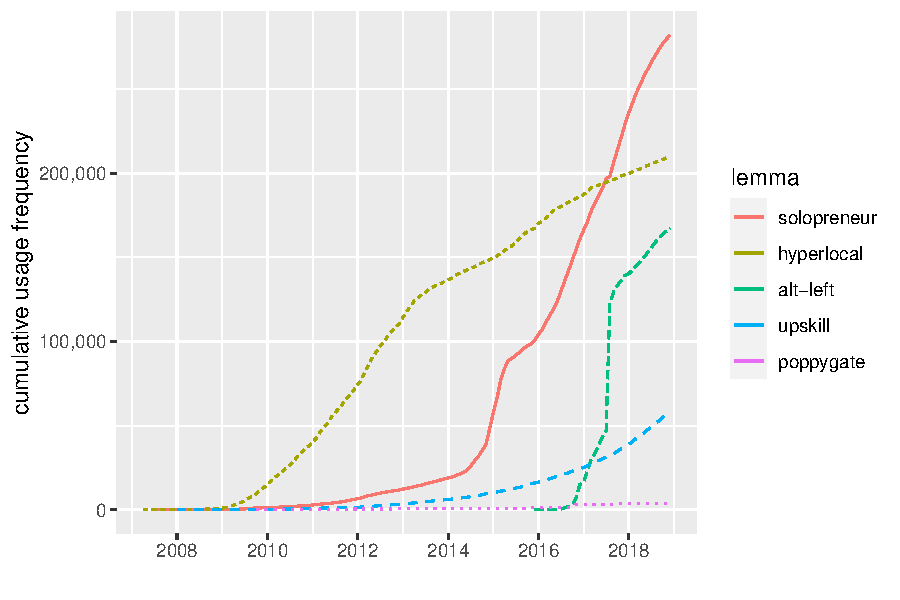
\includegraphics[width=\linewidth, height=.8\textheight, keepaspectratio]{img/freq_cum_cases.pdf}
        \caption{Cumulative increase in usage frequency for case studies.\protect\footnotemark}
        \label{fig:freq_cum_cases}
      \end{figure}
      \footnotetext{\ol{alt-right} was omitted from this plot because its high usage frequency would have inhibited the interpretability of the other lexemes; its frequency over time is presented in Figure \ref{subfig:freq_temp_alt-right}.}

      While the end points of the trajectories in Figure~\ref{fig:freq_cum_cases} mark the target words' total frequency counts as shown in Table~\ref{subtab:freq-total-cases}, the offsets and slopes of the trajectories of usage frequency reveal additional characteristics about differences in their diffusion patterns.

      The selected cases differ regarding their total lifespan observed, which is indicated by diverging starting points of diffusion. The term \ol{hyperlocal}, for example, is the oldest new word among the selected cases, and it is commonly used to refer to information that has a strong focus on local facts and events. While it was hardly used in the first years of Twitter, it started to increase in its use in 2009, and it was added to the OED's Third Edition in 2015. Around this time, the neologism \ol{solopreneur} only started to significantly increase in its use. A blend of \ol{solo} and \ol{entrepeneur}, it keeps a low, flat trajectory of sporadic use for about 7 years after its first appearance in the corpus. The first two attestations in the corpus indicate the sense of novelty and scepticism towards the term in its early phases:

      \renewcommand{\labelenumi}{(\arabic{enumi})}
      \begin{enumerate}
        \item I'm trying to figure out if I like the term \enquote{solopreneur} I just read. (27 July, 2007)
        \item hmmmmmmm new word added to my vocab = \enquote{solopreneur} !! (6 January, 2008)
      \end{enumerate}

      Most speakers increasingly \enquote{like the term} and \enquote{add them to their vocabulary} only much later, after 2014, when the phenomenon of individual entrepreneurship attracts increasing conceptual salience in the community, which seems to be both reflected and propagated by the publication of several self-help books for entrepreneurs in this year, which all explicitly use this new term in their titles (e.g. the popular guide \emph{Free Tools for Writers, Bloggers and Solopreneurs} by Karen Banes). The following short, but intense period of use results in a higher overall number of uses for \ol{solopreneur} as compared with \ol{hyperlocal}, even though the use of the latter term shows a longer lifespan of continual use.

      In addition to lifespan differences, the slopes of the cumulative trajectories in Figure~\ref{fig:freq_cum_cases} indicate differences regarding the dynamics of diffusion underlying the aggregated total number of uses over time.

      Neologisms such as \ol{hyperlocal} and \ol{upskill} (\enquote{to learn new skills}) show a steady, gradual increase in usage frequency over longer periods of time. By contrast, the use of other candidates such as \ol{solopreneur} and \ol{alt-left} is much less stable and evenly distributed over time.

      In the case of \ol{solopreneur}, we observe a big spike in frequency following its increased popularity in the entrepreneurial community in 2014. While it shows the highest total frequency count in Figure~\ref{fig:freq_cum_cases}, the majority of its uses fall into the second part of its observed lifespan.

      An even shorter and steeper increase can be seen in the use of \ol{alt-left}, which is the youngest neologism to enter the scene at the end of 2015. \ol{alt-left} was coined as a counterpart to the term \ol{alt-right}. The latter neologism is a shortening of \ol{Alternative Right}, which was introduced by the white-supremacist Richard Spencer in 2010 as a new umbrella term for far-right, white nationalist groups in the United States. Facing substantial criticism for racist attitudes and actions, proponents of this far-right political camp coined and attempted to propagate the derogatory term \ol{alt-left} to disparage political opponents. Despite its late appearance in the corpus, \ol{alt-left} occurs in a total of \num{163809} tweets, which places it in the medium range of the sample in terms of total frequency counts. However, its trajectory in Figure~\ref{fig:freq_cum_cases} shows that the majority of its use goes back to a single period of highly intensive use in the second half of 2017, soon after which it slows down considerably.

      The cumulative increase in usage intensity of the selected cases illustrates that similar total frequency counts of neologisms can be the product of highly different pathways of diffusion.

      These data complement total counts in that they show differences in the total lifespan and in the intensity and with which a neologism was used over time, which is relevant for assessing the degree to which it has spread in the speech community.


    \subsubsection{Absolute frequency}

      Going beyond cumulative counts, absolute usage frequency counts provide a more more-grained view of the temporal dynamics of diffusion.

      \marginpar{\textsc{lifespan} should be discussed here; with reference to diffusion cut-offs; for later evaluation of SNA metrics}
      \marginpar{potentially also a table for \textsc{lifespan}: case studies, top k, bottom k}

      Most importantly, analysing usage intensity highlights to which degree new words are being used consistently over time. Figure \ref{fig:freq-abs} presents this information for the selected cases. In the following section, I will illustrate prototypical differences by referring to the selected cases, before I discuss the results for the full sample.

      \begin{figure}
        \centering
        \begin{subfigure}{.3\linewidth}
          \caption{\ol{upskill}}
          \label{subfig:freq_temp_upskill}
          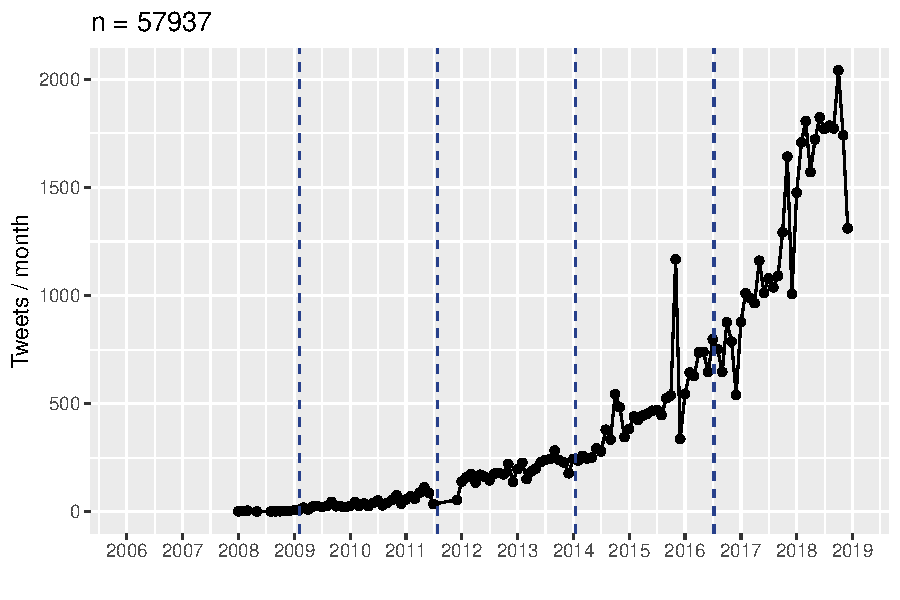
\includegraphics[width=\linewidth, height=.8\textheight, keepaspectratio]{"img/ui_upskill_time.pdf"}
        \end{subfigure}
        \begin{subfigure}{.3\linewidth}
          \caption{\ol{hyperlocal}}
          \label{subfig:freq_temp_hyperlocal}
          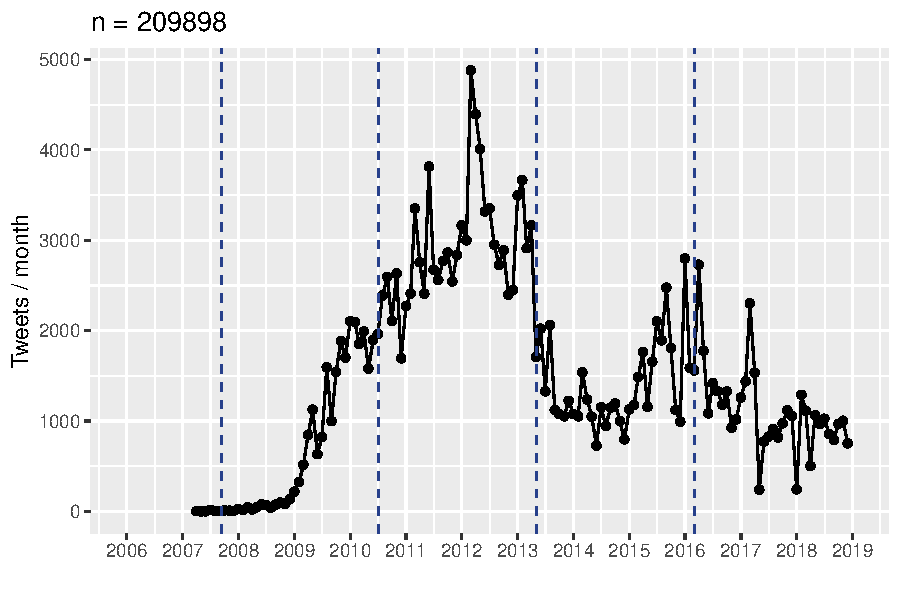
\includegraphics[width=\linewidth, height=.8\textheight, keepaspectratio]{"img/ui_hyperlocal_time.pdf"}
        \end{subfigure}
        \begin{subfigure}{.3\linewidth}
          \caption{\ol{solopreneur}}
          \label{subfig:freq_temp_solopreneur}
          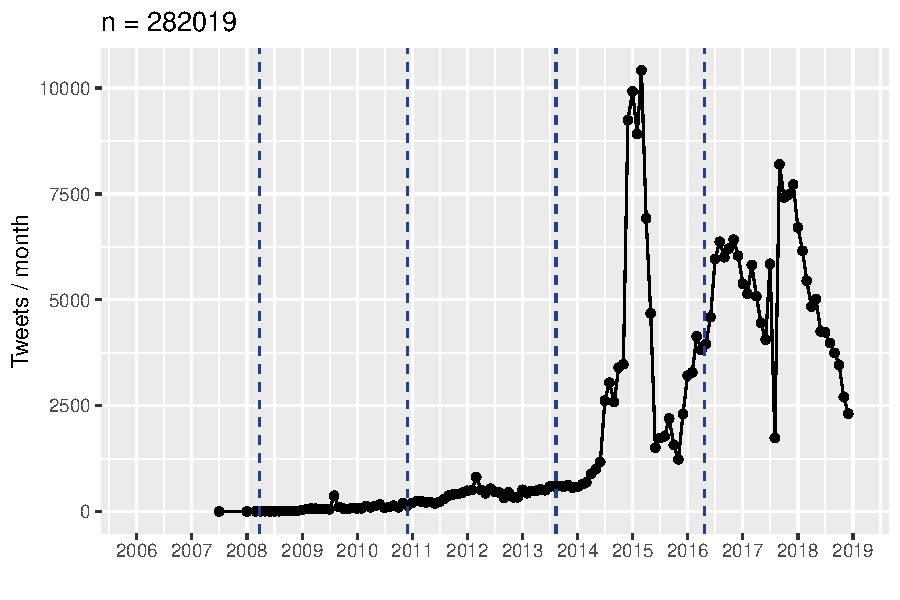
\includegraphics[width=\linewidth, height=.8\textheight, keepaspectratio]{"img/ui_solopreneur_time.pdf"}
        \end{subfigure}

        \begin{subfigure}{.3\linewidth}
          \caption{\ol{alt-right}}
          \label{subfig:freq_temp_alt-right}
          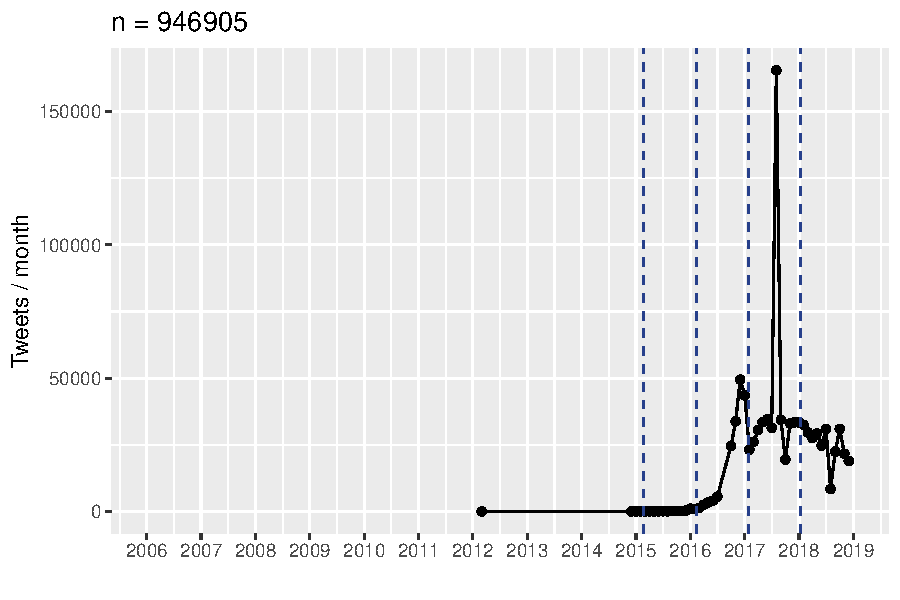
\includegraphics[width=\linewidth, height=.8\textheight, keepaspectratio]{"img/ui_alt-right_time.pdf"}
        \end{subfigure}
        \begin{subfigure}{.3\linewidth}
          \caption{\ol{alt-left}}
          \label{subfig:freq_temp_alt-left}
          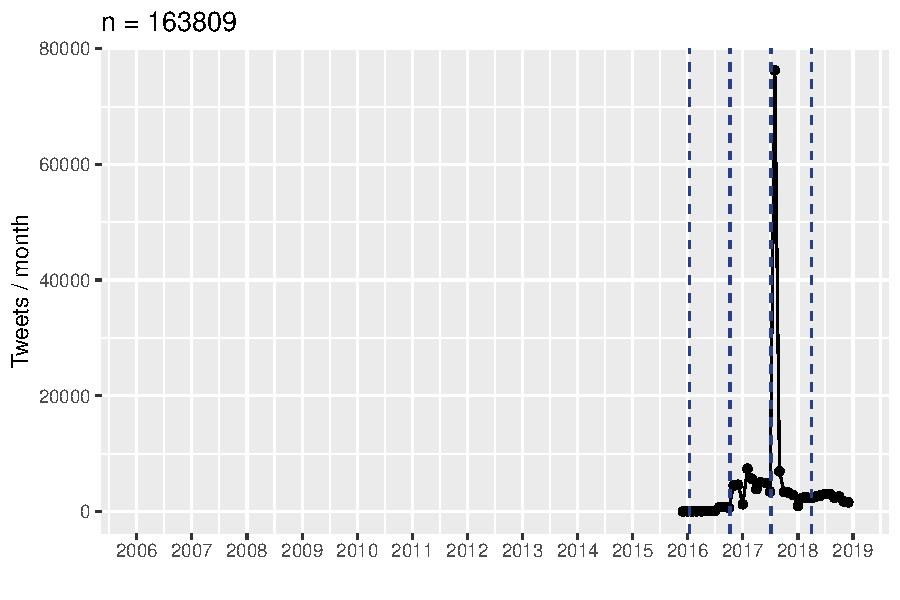
\includegraphics[width=\linewidth, height=.8\textheight, keepaspectratio]{"img/ui_alt-left_time.pdf"}
        \end{subfigure}
        \begin{subfigure}{.3\linewidth}
          \caption{\ol{poppygate}}
          \label{subfig:freq_temp_poppygate}
          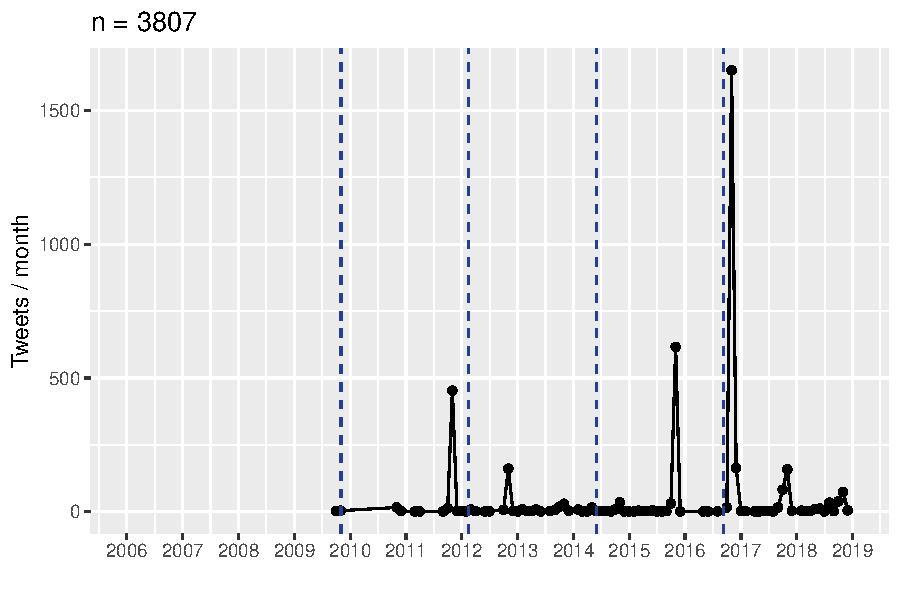
\includegraphics[width=\linewidth, height=.8\textheight, keepaspectratio]{"img/ui_poppygate_time.pdf"}
        \end{subfigure}
        \caption{Temporal dynamics in usage frequency for the case study neologisms.}
        \label{fig:freq-abs}
      \end{figure}

      The absolute frequency plots confirm differences regarding the lifespan and dynamics of usage intensity among the neologisms discussed above. In terms of lifespan, Figure \ref{fig:freq-abs} shows that \ol{upskill} and \ol{hyperlocal} are much older than \ol{alt-right} and \ol{alt-left}. The absolute counts also highlight the fact that while there is a low level of use of \ol{solopreneur} since 2007, its main period of diffusion starts much later, in 2014, with a subsequent spike in usage intensity.

      \qpar{Volatility}

        Besides, the absolute frequency counts over time provide a more detailed picture of the temporal dynamics of use. While the cumulative counts in Figure \ref{fig:freq_cum_cases} suggest smooth trajectories, the plots in Figure \ref{fig:freq-abs} indicate that the selected cases differ significantly in terms of the consistency with which they are used in the corpus.

        \marginpar{gradual increase} The neologism \ol{upskill} shows the smoothest trajectory of diffusion among the candidate neologisms. Aside from two smaller spikes, at the end of 2016 and 2018, it has gradually increased in its use since its first attestation in the corpus at the end of 2007. Neither its frequency counts, nor the corpus data suggest that its spread was triggered or propagated by specific topical events or the determining influence of individual influential users or user groups. After a long period of very slow, but consistent increase in frequency, its diffusion has accelerated in recent years. While its future remains uncertain, its previous trajectory resembles most closely the earlier phases of spread as predicted by S-curve models.

        \marginpar{consistent use} While \ol{hyperlocal} also exhibits a marked increase in usage frequency during its earlier stages, its peak of popularity is followed by a decline in use, after which it settles at a relative stable level of about \num{1000} tweets per month. This coincides with the OED's decision to take up \ol{hyperlocal} in its 2015 edition. Despite fluctuations, \ol{hyperlocal} has been used relatively consistently in the recent past, and seems to attract a stable community of users on Twitter.

        \marginpar{inconsistent use} The neologisms \ol{solopreneur} has been in use since 2007 and shows an overall increase in usage frequency, but its use fluctuates more strongly than that of \ol{hyperlocal}. After its initial peak around 2015, which coincides with the release of several self-help books featuring the term, its frequency plummets, becomes less stable, and shows an overall downward trend.

        \marginpar{topicality} As was mentioned above, \ol{alt-right} and \ol{alt-left} are closely related. Both terms show high levels of volatility in their usage frequency. The former, older term showed significant diffusion in 2016, particularly in the period following up to Donald Trump's election, after which \ol{alt-right} was consistently used to a relatively high degree, at about \num{25000} comments per month. Its counterpart, \ol{alt-left}, enters the scene much later, during the infamous Charlottesville Rally in 2017, whose topical effect causes a huge spike in the use of both terms. However, unlike \ol{alt-right}, which returns to its previous usage intensity, the use of \ol{alt-left} seems to largely disappear from Twitter in the aftermath of the event.

        \marginpar{recurrent topicality} The last example among the selected candidates, \ol{poppygate}, also exhibits high degrees of volatility, and it features the most distinctive pattern of spikes in its usage intensity. Unlike the single topical spike for \ol{alt-right} and \ol{alt-left}, its use follows a recurrent, regular pattern: speakers use it almost exclusively around Remembrance Day, which takes place in November. The term \ol{poppygate} represents a last category of neologisms in the sample, which show wide fluctions in usage intensity, but for which these patterns follow a regular temporal pattern. \marginpar{\enquote{topicality}~\parencite{Fischer1998LexicalChange}; \enquote{recurrent semi-conventionalization}~\parencite{Kerremans2015WebNew})}


    \subsubsection{Coefficient of variation}

      To quantify the degree to which neologisms are used with consistent frequency over time, I calculate and compare the coefficients of variation for each neologism in the sample. This metric captures the overall variation in usage frequency of words over their lifespan relative to their average frequency of occurrence in the corpus. Table~\ref{tab:coef-var} presents the coefficients of variation for the selected cases, as well as for the top and bottom six neologisms that show the highest and lowest degrees of variation in the sample.

      \begin{table}
        \caption{Coefficients of variations.(\textsc{var})\protect\footnotemark}
        \label{tab:coef-var}
        \centering
        \begin{subtable}[t]{.3\linewidth}
          % \centering
          \begin{tabular}{
              l
              S[table-format=1.2, round-mode=places, round-precision=2]
            }
            \toprule
            Lexeme      & \textsc{var} \\
            \midrule
            hyperlocal  & 0.9783703    \\
            upskill     & 1.1399599    \\
            solopreneur	& 1.2046616    \\
            alt-right   & 1.8054940    \\
            poppygate   & 4.7535750    \\
            alt-left    & 5.3112621    \\
            \bottomrule
          \end{tabular}
          \caption{Variation among the selected cases.}
          \label{subtab:coef-var-cases}
        \end{subtable}
        \hfill
        \begin{subtable}[t]{.3\linewidth}
          % \centering
          \begin{tabular}{
              l
              S[table-format=1.2, round-mode=places, round-precision=2]
            }
            \toprule
            Lexeme      & \textsc{var} \\
            \midrule
            followership  & 0.7147413 \\
            lituation     & 0.7174908 \\
            twitterverse  & 0.7215036 \\
            detweet       & 0.7436056 \\
            remoaners     & 0.7605029 \\
            twittersphere & 0.7670257 \\
            % baecation   & 0.7705697 \\
            % foodventure & 0.7714314 \\
            % broette     & 0.7726448 \\
            % upcycling   & 0.7995218 \\
            \bottomrule
          \end{tabular}
          \caption{Lowest degrees of variation.}
          \label{subtab:coef-var-lowest}
        \end{subtable}
        \hfill
        \begin{subtable}[t]{.3\linewidth}
          % \centering
          \begin{tabular}{
              l
              S[table-format=1.2, round-mode=places, round-precision=2]
            }
            \toprule
            Lexeme      & \textsc{var} \\
            \midrule
            upskirting    & 9.3861492 \\
            youthquake    & 6.3218380 \\
            alt-left      & 5.3112621 \\
            birther       & 5.0001924 \\
            poppygate     & 4.7535750 \\
            cherpumple    & 4.6909168 \\
            % climate     & 14752     \\
            % incel       & 3.0090748 \\
            % neckbuds    & 2.9861481 \\
            % bloggergate & 2.7765687 \\
            \bottomrule
          \end{tabular}
          \caption{Highest degrees of variation.}
          \label{subtab:coef-highest}
        \end{subtable}
      \end{table}
      \footnotetext{Neologisms with a lifespan shorter than one year and/or less than \num{2000} comments ($n = 5$) were excluded since the coefficient of variation does not provide robust measures for these short-lived, infrequent outliers.}

      The results in Table~\ref{tab:coef-var} show that the sample covers a wide spectrum of variability in usage frequency.

      Among the neologisms that were used the most consistently, i.e. exhibit the lowest degrees of variation, we find words whose frequency-based measures suggested high degrees of conventionality. For example, \ol{twitterverse} is listed among the most frequent neologisms in Table~\ref{subtab:freq-total-max} and is also one of the oldest neologisms, with its first attestation in the corpus dating back to 19 December, 2006.

      By contrast, the group of lexemes that show the highest degree of variation in usage frequency is comprised by neologisms with lower degrees of conventionality, which are generally less frequent and were coined more recently. Notably, topical spikes play a crucial role in the diffusion processes of all examples in this category: the diffusion of \ol{alt-left} and \ol{birther}\footnote{\enquote{proponent of the \enquote{birther movement}, a conspiracy theory which claims that President Obama's birth certificate was forged, and that he was not born in the USA.}} was promoted by extralinguistic political events, \ol{upskirting}\footnote{\mn{The habit or practice of taking upskirt photographs or videos.} (OED)} and \ol{youthquake}\footnote{\mn{a significant cultural, political, or social change arising from the actions or influence of young people} (\url{https://languages.oup.com/word-of-the-year/2017/})} were advanced through increased metalinguistic salience after they were added to the OED and awarded Word of the Year 2017 by Oxford University Press. Both \ol{poppygate} and \ol{cherpumple}\footnote{\mn{Cherpumple is short for cherry, pumpkin and apple pie. The apple pie is baked in spice cake, the pumpkin in yellow and the cherry in white.} (\url{https://en.wikipedia.org/wiki/Cherpumple}); typically consumed during the holiday season in the US.} exhibit recurrent topicality, and are typically only used in the contexts of their seasonal relevance in autumn and winter.

      The selected cases cover the spectrum of variability in usage frequency found in the full sample of neologisms, and the coefficients of variation are in line with the previous analysis of the frequency-based time-series visualisations presented in Figure~\ref{fig:freq-abs}.


      \subsubsection{Summary of frequency-based measures}

        So far, I have used frequency-based visualisations and metrics to assess the degrees and pathways of diffusion of the neologisms in the sample. In a first step, I used the most common measure for assessing the conventionality of new words: their total frequency of occurrence in the corpus. In the following steps, I extended the frequency-based approach by including temporal information in the analysis. Zooming in on the temporal dynamics of use surfaced different pathways of diffusion. Notably, it revealed substantial differences in the diachronic usage profiles of neologisms with comparable total frequency.

        \marginpar{total frequency} Within the group of selected cases, \ol{hyperlocal}, \ol{solopreneur}, and \ol{alt-left}, for example, would all be placed in the medium range of the conventionality continuum if grouped by total usage frequency alone, as presented in Table~\ref{subtab:freq-total-cases}. Taking this most basic measure as an indicator of degrees of diffusion, it would seem that these words are roughly equally conventional among users on Twitter. However, adding the temporal dynamics of their use in the corpus to the picture revealed significant differences between their diachronic usage profiles, which seems important for assessing their pathways and degrees of diffusion in a more differentiated and accurate way.

        Visualising the cumulative increase in uses over time (Table~\ref{fig:freq_cum_cases}) for \ol{hyperlocal}, for example, shows a stable linear trend, which indicates that its total frequency count has been the product of relatively consistent use over its relatively long lifespan. Its temporal usage profile in Figure~\ref{subfig:freq_temp_hyperlocal} and confirms these observations and presents its initial period of accelerated diffusion followed by an extended stable level of relatively consistent use over the last five years of its observed lifespan. This consistency is further corroborated by its low coefficient of variation (Table~\ref{subtab:coef-var-cases}). In sum, the balanced nature of this frequency-based usage profile suggests a relatively organic trajectory of diffusion, culminating in a solid degree of conventionality in the recent past. The fact that \ol{hyperlocal} was added to the OED in 2015 supports these observations.

        By comparison, \ol{solopreneur} has a slightly higher overall frequency of occurrence, yet its use is less stable over time. I

          results
            higher total frequency counts
            trend
              rapid surge of diffusion
              followed by a slightly negative, concave trend in its later stages
            lifespan
            variation in use: strong

          diffusion and conventionalization
            pathway: topical
            degree: limited

        \marginpar{alt-left}

          results
            trend
              explosion: Featuring an even more extreme spurt of diffusion, the use of \ol{alt-left} explodes in August 2017,
              implosion: yet its popularity quickly vanishes soon after, and it seems to attract very little popularity among the majority of speakers after that.

            lifespan: young
            variation: the highest
          diffusion and conventionalization
            pathway: topical
            degree: limited


      open questions
        how many
        users?
        user groups?
    --> social network analysis




going beyond frequency

  results

    total frequency $\neq$ number users/communities
      similar counts, different underlying temporal patterns (trend, lifespan, volatility)
    frequency time-series
      slopes (trend)
        gradual diffusion: \ol{upskill}
      lifespan
        overestimate: obsolete: \ol{millenium bug}
        underestimate: new, but established: \ol{coronavirus}
      volatility
        one-hit wonders: \ol{alt-left}
        consistent use: \ol{hyperlocal}

  particularly important for \emph{lexical} \emph{innovations} due to the nature of the process

    bound to cultural conceptual salience (variable \enquote{semantic carrying capacity}~\parencite{Nini2017ApplicationGrowth})
    social indexicality
    open nature of the lexicon


  full sample

  stability: shows that freq. is problematic
    \enquote{dormant}
    spikes distort representativity of frequency for degree of conventionality
      In this case, a less steady, more abrupt increase in usage over a relatively short period as with \ol{solopreneur} could be a sign of high usage intensity within one community (\enquote{usualization}), rather than an indication of sustained spread to larger numbers of other speakers and communities (\enquote{diffusion}).
    underestimate: \ol{poppygate} not forgotten in troughs
    overestimate: cumulating hides the fact that words like \ol{millenium} do get lost


  going beyond frequency

    In the following sections I will assess the value of usage frequency and compare and complement it with social network information about the diffusion of lexical innovations.

  \subsection{Social networks of diffusion}
    \label{subsec:sna}

    \subsubsection{Centralization over time}

  going beyond frequency

  def. diffusion:
    numbers of users
    communities

  subsetting / time slices
    start of diffusion process
    4 quarters

  explain: degree centralization

  case studies
    example where freq. meets nets
    example where nets add to freq.: \ol{alt-left}

      \qpar{Overview of changes in centralization for case studies.}

      \begin{figure}[H]
        \caption{Degree centralization over time for case study words.}
        \centering
        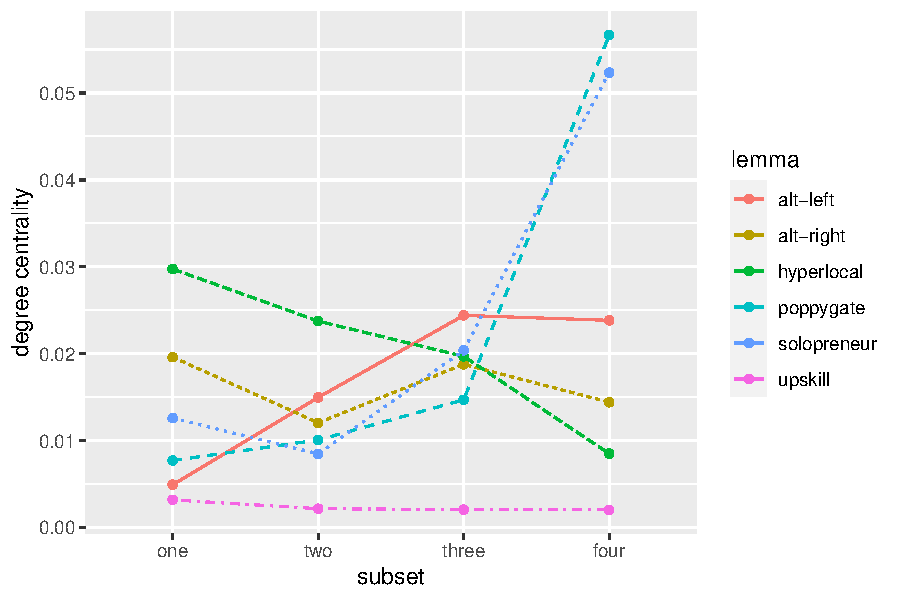
\includegraphics[width=\linewidth, height=.8\textheight, keepaspectratio]{img/cases_cent_diac.pdf}
      \end{figure}

      \qpar{Advanced / increasing: \ol{hyperlocal}}

      \begin{figure}[H]
        \caption{Social network of diffusion for \ol{hyperlocal} over time.}
        \centering
        \begin{subfigure}{.45\linewidth}
          \caption{First stage}
          \centering
          \includegraphics[width=\linewidth]{example-image-a}
          % \includegraphics[width=\linewidth, height=\textheight, keepaspectratio]{../gephi/plots/hyperlocal_one.pdf}
        \end{subfigure}
        \begin{subfigure}{.45\linewidth}
          \caption{Second stage}
          \centering
          \includegraphics[width=\linewidth]{example-image-b}
          % \includegraphics[width=\linewidth, height=\textheight, keepaspectratio]{../gephi/plots/hyperlocal_two.pdf}
        \end{subfigure}\\
        \begin{subfigure}{.45\linewidth}
          \caption{Third stage}
          \centering
          \includegraphics[width=\linewidth]{example-image-c}
          % \includegraphics[width=\linewidth, height=\textheight, keepaspectratio]{../gephi/plots/hyperlocal_three.pdf}
        \end{subfigure}
        \begin{subfigure}{.45\linewidth}
          \caption{Fourth stage}
          \centering
          \includegraphics[width=\linewidth]{example-image-a}
          % \includegraphics[width=\linewidth, height=\textheight, keepaspectratio]{../gephi/plots/hyperlocal_four.pdf}
        \end{subfigure}
      \end{figure}

      \qpar{Limited / limited: \ol{alt-left}}

      \begin{figure}[H]
        \caption{Social network of diffusion for \ol{alt-left} over time.}
        \centering
        \begin{subfigure}{.45\linewidth}
          \caption{First stage}
          \centering
          \includegraphics[width=\linewidth]{example-image-a}
          % 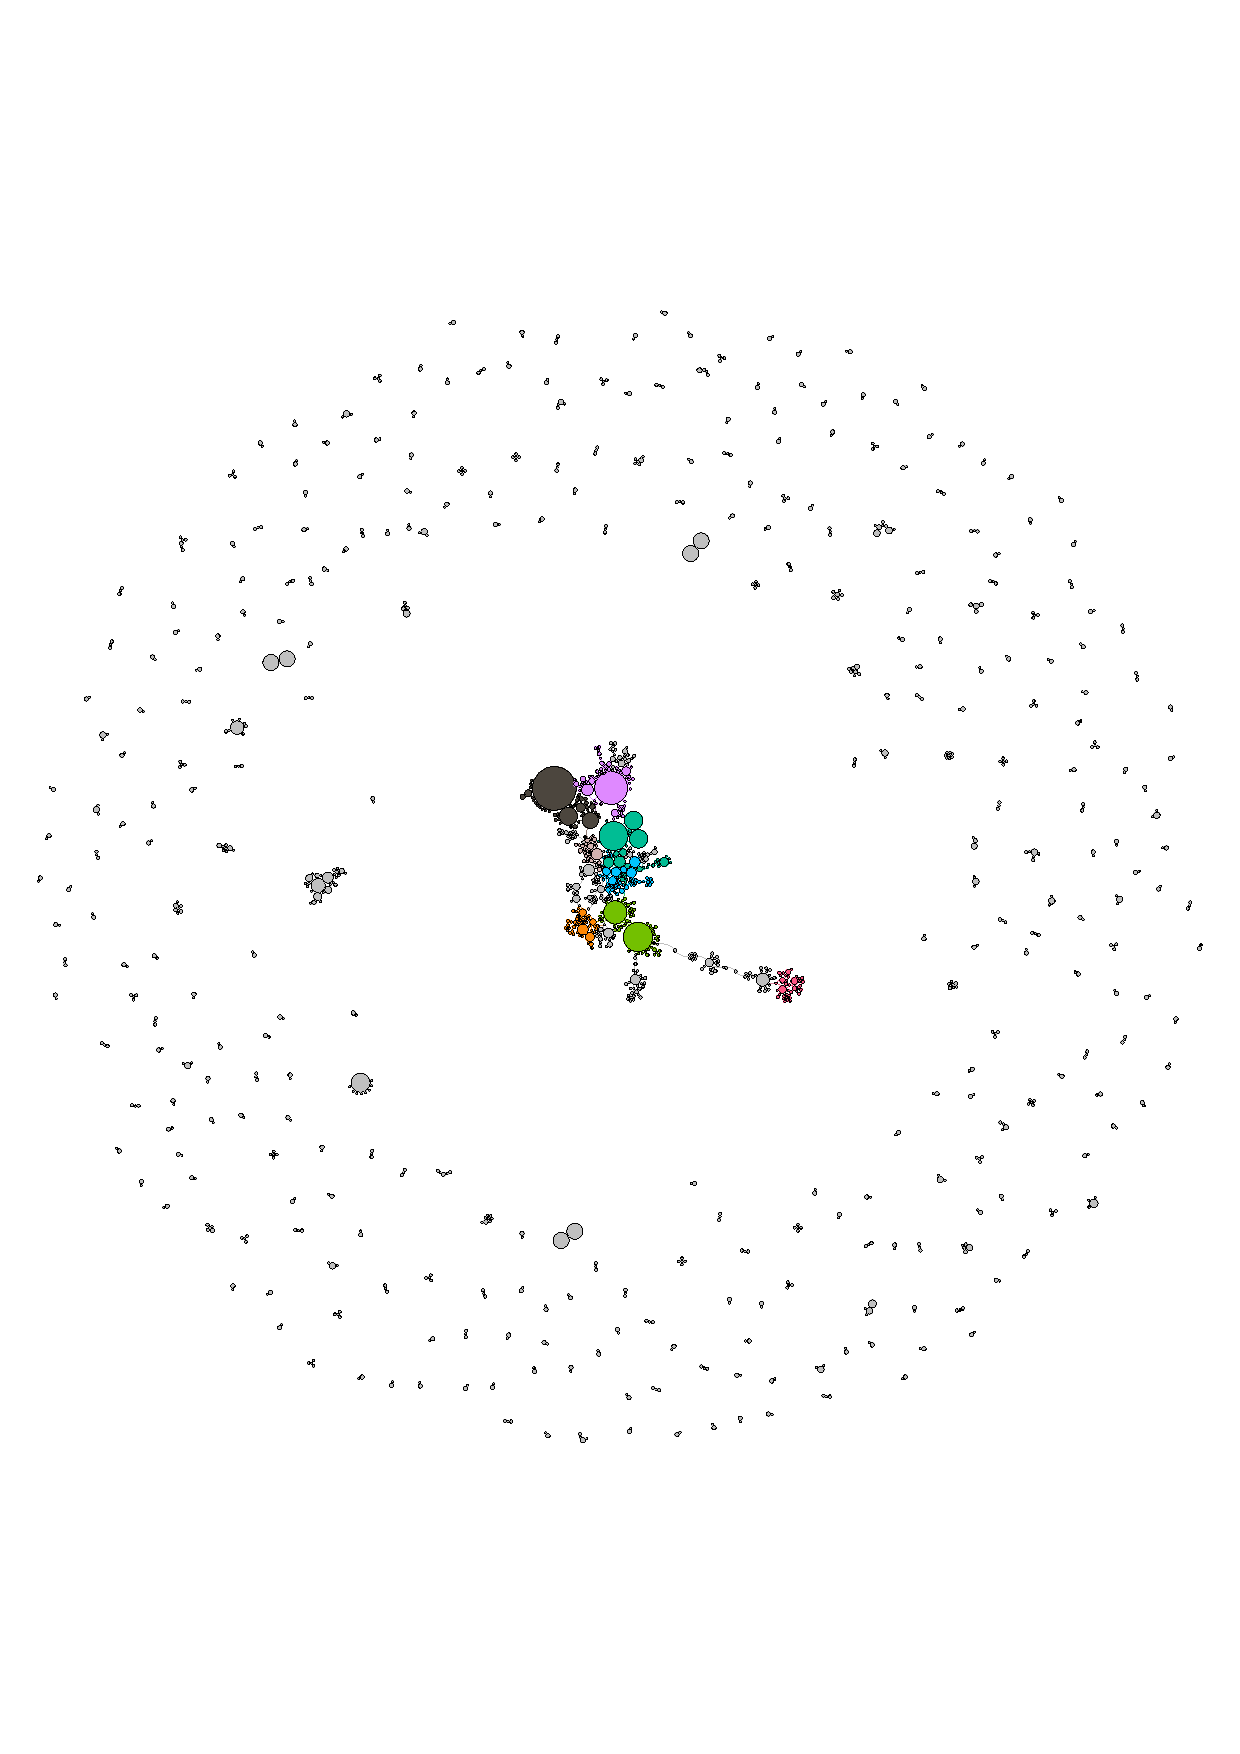
\includegraphics[width=\linewidth, height=\textheight, keepaspectratio]{../gephi/plots/alt-left_one.pdf}
        \end{subfigure}
        \begin{subfigure}{.45\linewidth}
          \caption{Second stage}
          \centering
          \includegraphics[width=\linewidth]{example-image-b}
          % 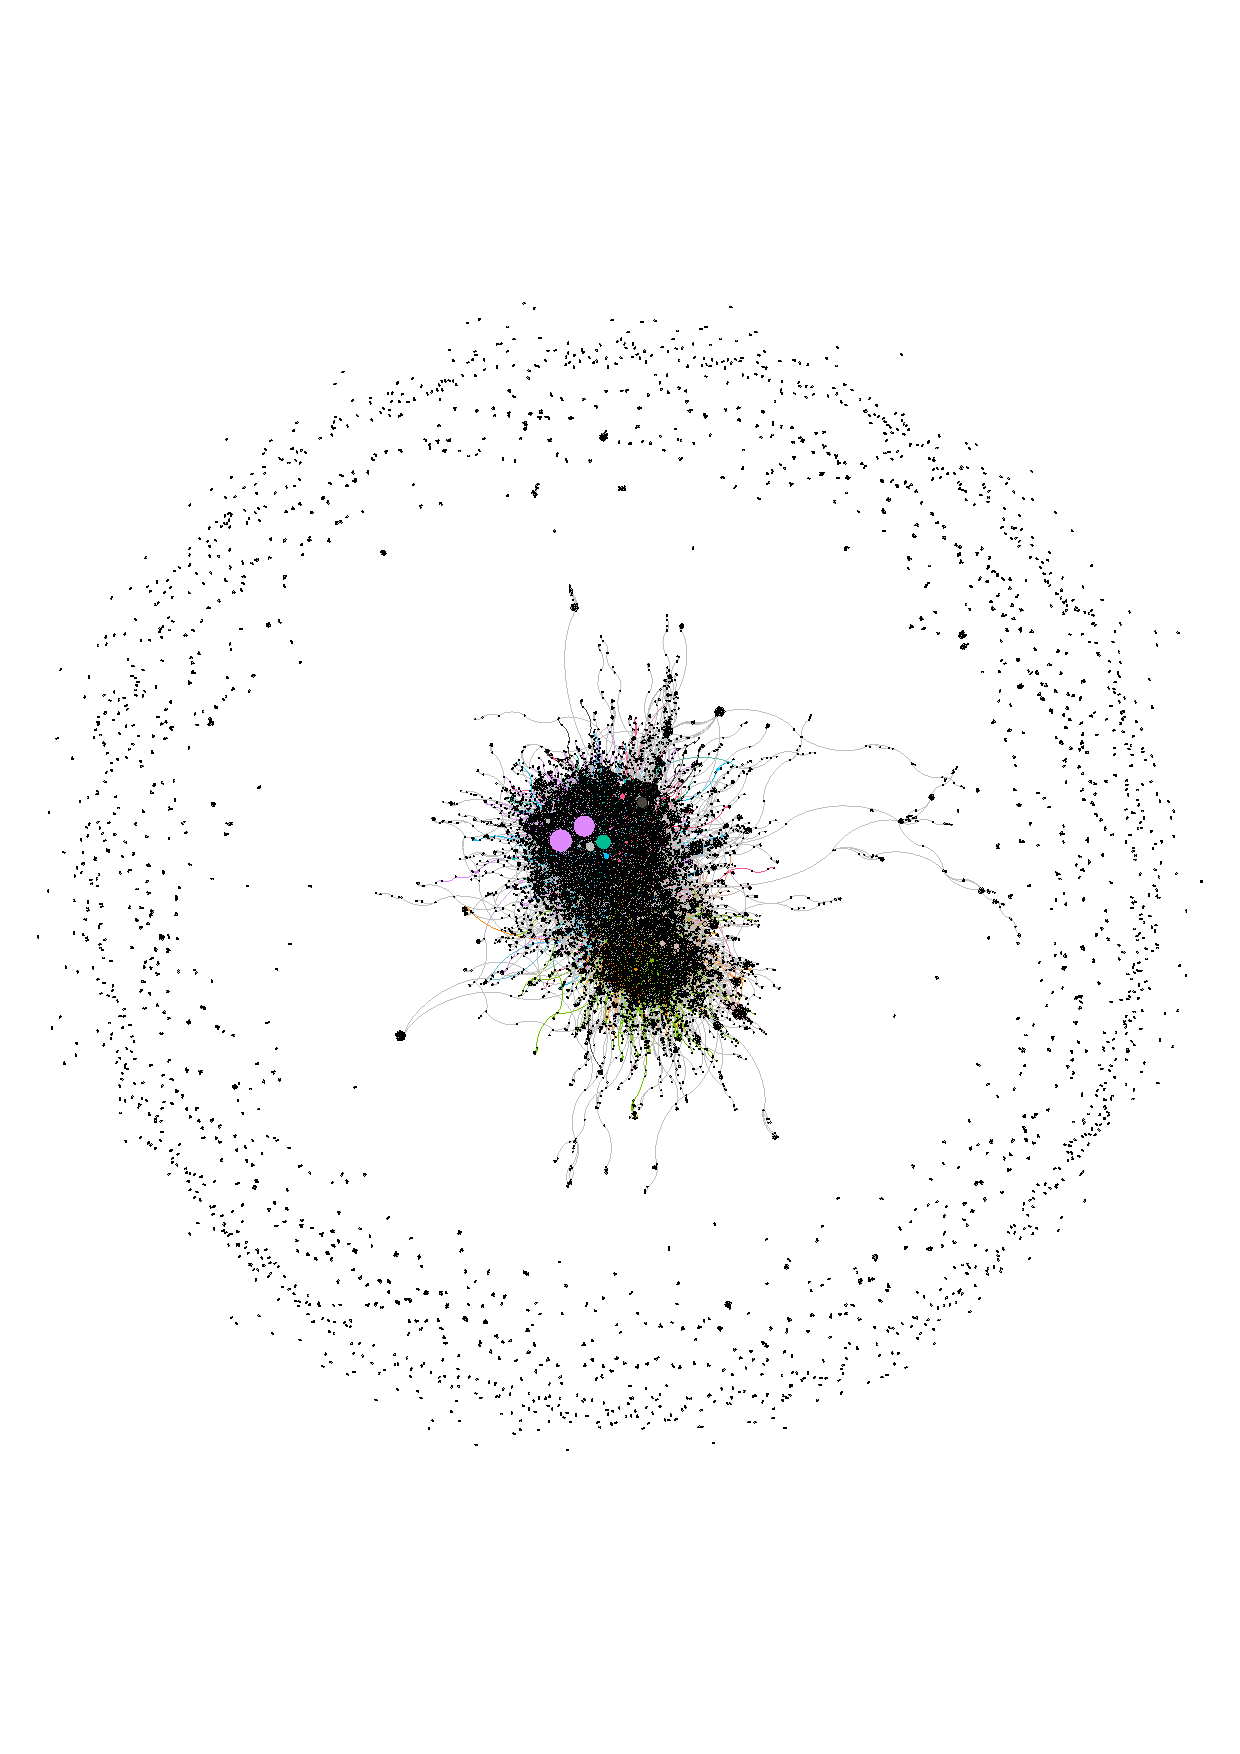
\includegraphics[width=\linewidth, height=\textheight, keepaspectratio]{../gephi/plots/alt-left_two.pdf}
        \end{subfigure}\\
        \begin{subfigure}{.45\linewidth}
          \caption{Third stage}
          \centering
          \includegraphics[width=\linewidth]{example-image-c}
          % \includegraphics[width=\linewidth, height=\textheight, keepaspectratio]{../gephi/plots/alt-left_three.pdf}
        \end{subfigure}
        \begin{subfigure}{.45\linewidth}
          \caption{Fourth stage}
          \centering
          \includegraphics[width=\linewidth]{example-image-a}
          % 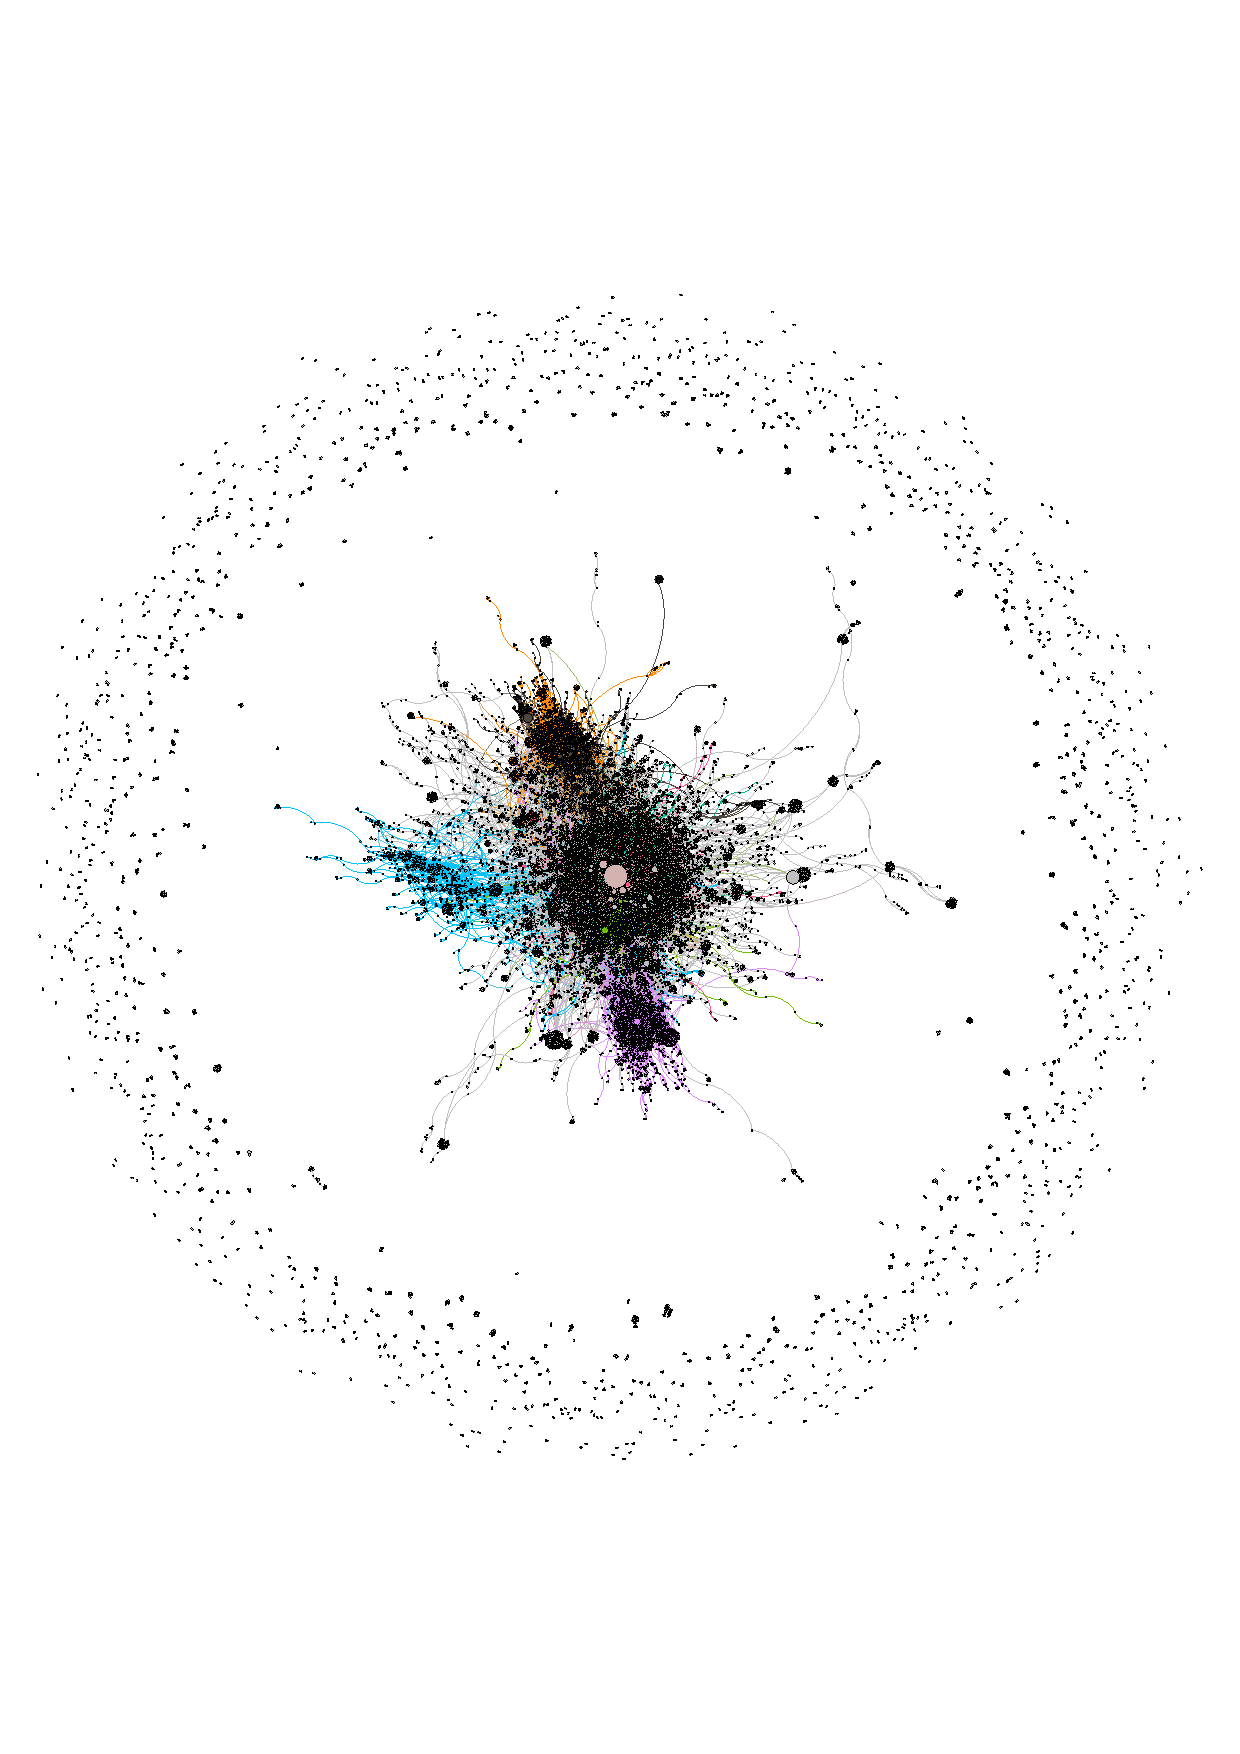
\includegraphics[width=\linewidth, height=\textheight, keepaspectratio]{../gephi/plots/alt-left_four.pdf}
        \end{subfigure}
      \end{figure}

      \qpar{Full sample}

  density
  successful
  unsuccessful

  biggest changes

    \subsubsection{Overall centralization}

  most diffused
  least diffused

  \subsection{Networks vs. frequency}
    \label{subsec:nets-vs-freq}

    \subsubsection{Correlation}
      \label{subsubsec:corr}

      \begin{table}[H]
        \centering
        \caption{Correlations of \textsc{centrality} (\enquote{degree centralization}) with the variables total usage frequency (\textsc{frequency}), coefficient of variation (\textsc{variation in frequency}), and observed lifespan (\textsc{lifespan}) across the full sample of neologisms ($n=100$); reporting correlation coefficients and \emph{p}-values for Spearman's $\rho$~\parencite{Spearman1961ProofMeasurement} and Kendall's $\tau$~\parencite{Kendall1938NewMeasure}.}
        \label{tab:correlations}
        \begin{tabular}{
          >{\scshape}l
          ||
          S[table-format=2.2, round-mode=places, round-precision=2]
          S[table-format=1.5, round-mode=places, round-precision=5]
          |
          S[table-format=2.2, round-mode=places, round-precision=2]
          S[table-format=1.5, round-mode=places, round-precision=5]
          }
          \toprule
          & \multicolumn{2}{c}{Spearman} & \multicolumn{2}{c}{Kendall} \\
          & $\rho$                       & p & $\tau$ & p              \\
          \midrule
          usage frequency        & -0.3974644 & 0.00005338 & -0.2743764 & 0.00005727 \\
          lifespan               & -0.2894037 & 0.003668   & -0.2029075 & 0.002932   \\
          variation in frequency & 0.2922202  & 0.003449   & 0.1956298  & 0.004118   \\
          \bottomrule
        \end{tabular}
      \end{table}


    \subsubsection{Discrepancies}
      \label{subsubsec:discrepancies}

  However, we also see discrepancies

  plots

  \begin{figure}[H]
    \centering
    \begin{subfigure}{.45\linewidth}
      \caption{Full sample.}
      \centering
      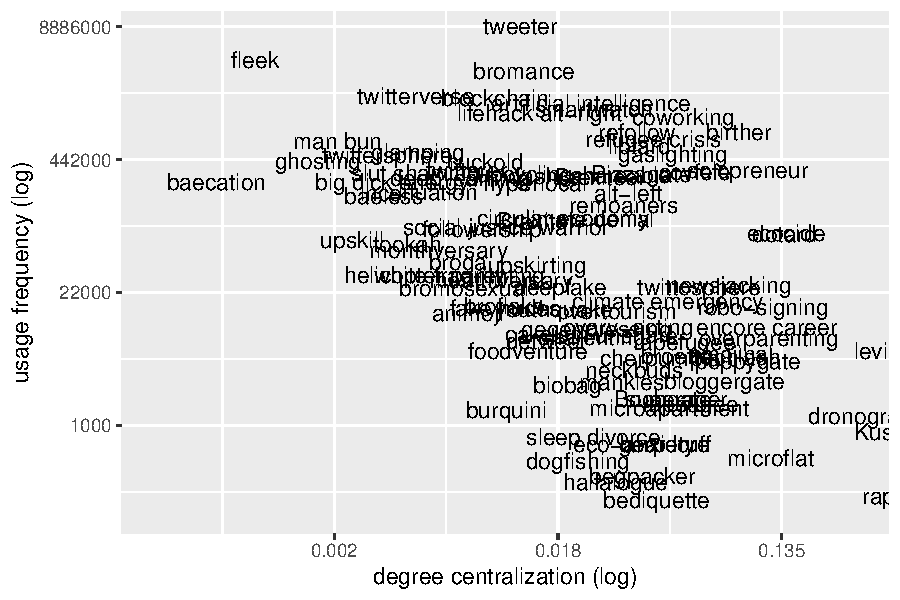
\includegraphics[width=\linewidth, height=.8\textheight, keepaspectratio]{img/full_cent_freq_overall.pdf}
    \end{subfigure}
    \begin{subfigure}{.45\linewidth}
      \caption{Case studies.}
      \centering
      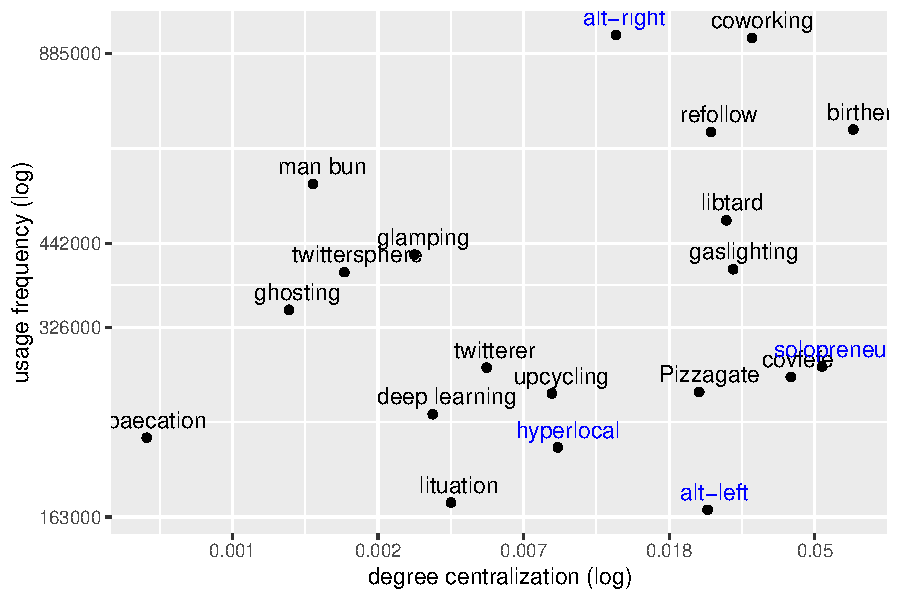
\includegraphics[width=\linewidth, height=.8\textheight, keepaspectratio]{img/cases_cent_freq_overall.pdf}
    \end{subfigure}
  \end{figure}

  cluster analysis

  freq. overestimating
  topical
  propaganda: \ol{alt-right}, \ol{alt-left}, \ol{covfefe}, \ol{birther}
  Brexit terms: \ol{Brexiteer}, \ol{Brexiter}, \ol{Brexit}
  nerds
  technical

  freq. underestimating: XXX
  topical words

  Social network metrics certainly add to freq.

\section{Discussion}
  \label{sec:discussion}

  %subsection{Summary}

    \begin{qitem}
      # I have investigated the diffusion of new words on Twitter.
      # I have focused on diffusion as regards the spread to new speakers and communities.
      # I have used frequency as a baseline and have gone beyond frequency to zoom in on the sociolinguistic dynamics of diffusion.
      # I have shown that Social Network Analysis can complement frequency measures
    \end{qitem}

  %subsection{Discussion}

    \begin{qitem}
      # freq. empirically proves to be a pretty good indicator

      # drawbacks of cumulated, total counts: temporal dynamics important

      # but rough approximation due to inferences
        ## active vs. passive use
        ## number of speakers
        ## groups of speakers

      # temporal dynamics important
        ## time window: age, lifespan
          ### starting point: late: very new words, would be under-represented by total counts
          ### end point: words might have already grown out of use (e.g. \ol{millenium bug}) > over-represented by total counts
          ### length: quick vs. slow and steady increase: topicality

        ## volatility: high topicality / highly fluctuating communicative need (cf. \ol{going to}-future); thus fluctuating ``semantic carrying capacity''~\parencite{Grieve2018MappingLexical}

      # dynamics in usage intensity might reflect social dynamics
        ## s. S-curve model: early adopters etc.
        ## e.g.: fast rise due to rapid spread in certain communities
        ## hard to infer from usage frequency > SNA needed

      # social network dynamics important
        ## esp. w.r.t. new words: often community-specific; are coined within tight-knit comminuties and (cf. grammatical change) and have socio-indexical function (e.g. youth language)
      # cross-validation between
      # cross-checking other data sources (NOW corpus) shows validity
      # social network analysis can be an important tool for sociolinguistics
        ## extend sociolinguistic research (on geographical variation; desideratum in \cite{Grieve2019MappingLexical})
    \end{qitem}

  %subsection{Directions for future work}

    \begin{qitem}
      # cross-validation of frequency and SNA information
        ## systematic comparison with web data, e.g. NOW corpus~\parencite{Davies2013CorpusNews}; early attempts:~\cite{Wurschinger2016UsingWeb}
        ## questionnaires; early work:~\cite{Kerremans2015WebNew}
      # investigation on diffusion across
        # contexts: different web registers~\parencite{Biber2016RegisterVariation}
        # cotexts: use word embeddings to study
          ## semantic innovation, meaning change
          ## and variation and change between communities~\parencite{Tredici2019YouShall} 
    \end{qitem}

\section{Conclusion}
  \label{sec:conclusion}

  Summary

    \begin{qitem}
      # I have investigated the diffusion of new words on Twitter.
      # I have focused on diffusion as regards the spread to new speakers and communities.
      # I have used frequency as a baseline and have gone beyond frequency to zoom in on the sociolinguistic dynamics of diffusion.
      # I have shown that Social Network Analysis can complement frequency measures
    \end{qitem}

  Importance of/for computational sociolinguistics

    \begin{qitem}
      # new data like Twitter
      # new methods like SNA, simulations, AI for embeddings
      # progress: ideas, scholars and progress will ``go viral''
    \end{qitem}

%section{Bibliography}

\printbibliography

\section*{Acknowledgements}

\begin{itemize}
  \item UI: Max, Fabi
  \item SNA: Kauermann group
  \item Hans-Jörg
\end{itemize}

\end{document}
